% !TEX root = ../thesis.tex

\chapter{Modeling of Multimode Superconducting Circuits: Circuit Quantization, Numerical Modeling, and Mode Preserving Transformations}\label{chp:circuit_quantization}



%================================================================
\section{Introduction}
%================================================================
Superconducting circuits with many interacting modes are increasingly common, and the first step in analyzing any such circuit is writing down its Hamiltonian.
Lumped-element circuit quantization provides a route from a circuit diagram to that Hamiltonian \cite{BurkardKochDiVincenzo2004,voolIntroductionQuantumElectromagnetic2017}, which several software packages now automate \cite{groszkowskiScqubitsPythonPackage2021a,chittaComputeraidedQuantizationNumerical2022a,rajabzadehAnalysisArbitrarySuperconducting2023,aumannCircuitQOpensourceToolbox2022,gelyQuCATQuantumCircuit2020}.

Whether by hand or in software, circuit quantization begins from the topology of a circuit, which sorts its degrees of freedom by the energies they carry.
A compact mode enters only through Josephson cosines, so its phase coordinate is periodic and its charge is quantized, as in the transmon.
An extended mode also carries inductive energy quadratic in phase, so its phase coordinate is real-valued, as in the fluxonium.
A harmonic mode carries only quadratic inductive and charging energy, as in an $LC$ resonator.
The remaining non-dynamical modes lack kinetic and/or potential energy and do not contribute to the dynamics of the circuit.

The topology dictates how many modes of each type there are, but it does not fix the coordinates that describe them.
Any invertible change of basis that respects the mode types gives an equally valid Hamiltonian, and automated tools generally pick one by a fixed rule.
This choice decides which couplings appear in the Hamiltonian, whether the Hamiltonians of different circuits can be easily compared, and how quickly a numerical diagonalization converges.
This chapter precisely characterizes transformations that preserve every mode type and poses the choice of coordinates as an optimization over them.

\Cref{sec:Lagrange} reviews flux-based quantization in a matrix formulation~\cite{voolIntroductionQuantumElectromagnetic2017,blaisCircuitQuantumElectrodynamics2021a,krantzQuantumEngineersGuide2019a,Ciani2024lecture}, with particular care for the cases of multiple compact modes and time-dependent external flux.
We quantize several compact modes on their joint lattice and give the irrotational flux assignment~\cite{YouKoch2019} in closed form, including loops broken by capacitors.
\Cref{sec:numerical_modeling} summarizes how the resulting Hamiltonians are diagonalized numerically.
\Cref{sec:Transforms} uses the framework of the previous section to define the class of mode-preserving transformations.
The choice of coordinates is then an optimization problem, which can be solved symbolically with general circuit parameters or numerically at fixed ones.
% We apply the technique to circuit enumeration~\cite{weissler2026enumerationsuperconductingcircuits5}, normal modes, and the KITE.
\Cref{sec:conc} concludes.


%=========================================================
\section{Multimode Circuit Quantization}\label{sec:Lagrange}
%=========================================================

We begin by reviewing circuit quantization of multimode superconducting circuits made of capacitors, inductors, and Josephson junctions.
Each ingredient appears in at least one existing review or software package~\cite{voolIntroductionQuantumElectromagnetic2017,blaisCircuitQuantumElectrodynamics2021a,krantzQuantumEngineersGuide2019a,rasmussenSuperconductingCircuitCompanionan2021a,groszkowskiScqubitsPythonPackage2021a,chittaComputeraidedQuantizationNumerical2022a,rajabzadehAnalysisArbitrarySuperconducting2023,Rajabzadeh2026generalframework,Wang2021,aumannCircuitQOpensourceToolbox2022,Ciani2024lecture,Lu2026systematic}.
Our goal is to present a concise but complete treatment that quantizes any multimode circuit of capacitors, inductors, and Josephson junctions.
Less common symbols used in this section are collected in \cref{tab:symbols}, with \cref{tab:notation} collecting all symbols for reference.
We retain time-dependent external flux, including through capacitively broken loops.
Which choices are conventions and which are required by the physics are clearly distinguished.
It should be noted that our treatment is restricted to the standard node flux formalism and does not allow for nonlinear capacitors or nonreciprocal elements.
More advanced methods \cite{osborne_symplectic_2023,OsborneFluxChargeSymmetricTheory2024,salcedoGyratorsSuperconductingCircuit2026,parra-rodriguez2023,parra-rodriguezExactQuantizationNonreciprocal2025, labarcaToolboxNonreciprocalDispersive2024} are required for these systems, but none have been implemented in an automated fashion.


\subsection{Constructing the Circuit Lagrangian}

We take a circuit to be fully specified by:
\begin{enumerate}
    \item {\bf Circuit branches}. $N_b$ circuit branches, each specifying a head and tail node, along with circuit elements and their parameters.
    \item {\bf A choice of ground node} or a floating circuit.
    \item {\bf Connections to voltage sources}. Classical voltage sources driving the circuit through coupling capacitors. Each voltage source connects to ground.
    \item {\bf Flux biases}. Loops threaded by external flux.
\end{enumerate}
Each passive branch carries a capacitance $C_k \geq 0$ and at most one inductor or Josephson junction.
Its contribution to the Lagrangian is
\begin{equation}
    \mathcal{L}_k = \frac{1}{2}C_k\dot\Phi_{b,k}^{\,2} - U_k(\Phi_{b,k}) \, ,
    \label{eq:branch_lagrangian_main}
\end{equation}
where $\dot\Phi_{b,k} = V_{b,k}(t)$ is the branch voltage and $\Phi_{b,k}  = \int_{-\infty}^t dt V_{b,k}(t)$ is the generalized branch flux.
\Cref{tab:branch_types} specifies the three passive branch types and their potentials.

\begin{table}[t]
\centering
\footnotesize
\setlength{\tabcolsep}{3pt}
\renewcommand{\arraystretch}{1.25}
\begin{tabular*}{\columnwidth}{@{\extracolsep{\fill}}lll@{}}
\toprule
Branch type & Parameters & $U_k(\Phi_{b,k})$ \\
\midrule
Linear capacitor & $C_k>0$ & $0$ \\[3pt]
Linear inductor & $L_k>0,\ C_k\geq0$ & $\Phi_{b,k}^{\,2}/(2L_k)$ \\[3pt]
Josephson junction & $E_{J_k}>0,\ C_k>0$ & $-E_{J_k}\cos(2\pi\Phi_{b,k}/\Phi_0)$ \\
\bottomrule
\end{tabular*}
\caption{Passive branch types and their branch-flux dependent energy contributions $U_k(\Phi_{b,k})$.
Capacitance contributes to the kinetic energy $T_{k} = \tfrac{1}{2}C_k\dot \Phi_{b,k}^2$ for every branch type.
Ideal voltage are treated separately and are fixed at $\dot\Phi_{b,k}=V_k(t)$.
Energies are in SI units, with $\Phi_0=h/(2e)$ being the superconducting flux quantum.}
\label{tab:branch_types}
\end{table}

The branch fluxes $\Phi_b$ are the physical circuit variables, but they are not independent when the circuit forms loops.
We describe the circuit loops by the loop matrix $\G$, whose $\ell$-th row has entries $\pm1$ on the branches around loop $\ell$, with signs set by each branch's orientation relative to the loop.
Every loop obeys Faraday's law, $\G\dot\Phi_b = \dot\Phi_{\rm ext}$, where $\Phi_{\rm ext}$ collects the external fluxes threading the loops.
Loops whose branches all carry an inductor or junction, the rows $\G_{JL}$, additionally obey fluxoid quantization, $\G_{JL}\Phi_b = \Phi_{\rm ext}$, with any integer fluxoid absorbed into $\Phi_{\rm ext}$.
For loops broken by a capacitor we fix the integration constant of Faraday's law in the same way, so all loops satisfy $\G\Phi_b=\Phi_{\rm ext}$.

To solve this constraint, we collect the fluxes of the $N$ internal circuit nodes in $\Phi$, excluding ground and prescribed voltage-source nodes.
The incidence matrix $\Omega$ maps node fluxes to branch differences.
Column $k$ corresponds to branch $k$ and has entries $+1$ at its head node and $-1$ at its tail node, with only the $+1$ for branches connecting to ground or a voltage source.
Node differences sum to zero around any loop, so $\G\Omega^T=0$ by definition, and $\Phi_b = \Omega^T\Phi$ is the general solution without external flux.
Adding a particular solution gives the full vector of branch variables
\begin{align}
    \Phi_b &= \Omega^T\Phi + \B\Phi_{\rm ext}\,, \qquad \G\B=I\,.
    \label{eq:branch_flux_main}
\end{align}
The flux assignment matrix $\B$ places the external fluxes on branches, with $[\B\Phi_{\rm ext}]_k$ being the flux assigned to branch $k$.
The constraint $\G\B=I$ ensures that each external flux offset is fully allocated and leaves $\B$ free up to $\B\to\B+\Omega^TM$ for any $N\times N_\ell$ matrix $M$.
This shift in $B$ is equivalent to an overall shift in the node variables $\Phi\to\Phi+M\Phi_{\rm ext}$.
We later use this freedom to simplify the Hamiltonian when external flux depends on time.

To build the lagrangian, we take the sum over branch variables. With the diagonal matrix $C_b$ containing the per-branch capacitance, the total capacitive energy in the circuit is $\tfrac{1}{2}\dot\Phi_b^T C_b \dot\Phi_b$.
It is typical to define the capacitance matrix $C = \Omega C_b \Omega^T$ to capture the node-flux dependent term of \cref{eq:branch_flux_main}.
Voltage sources and the external-flux dependent term both contribute to an offset charge
\begin{align}
    Q_g(t) = -C_V V(t) + \Omega C_b \B\dot\Phi_{\rm ext}(t) \, ,
    \label{eq:Q_g_node}
\end{align}
where the source-coupling matrix $C_V$ has entry $(i,s)$ equal to the total capacitance connecting node $i$ to voltage source $s$, and $V(t)$ gives the voltages of the classical source nodes.
The Lagrangian is the sum of these terms
\begin{align}
    \mathcal{L}(\Phi,\dot\Phi) &= \frac{1}{2}\dot\Phi^TC\dot\Phi + \dot\Phi^T Q_g(t) - \mathcal{U}(\Phi) \, ,
    \label{eq:L_node_standard}
\end{align}
plus the flux-dependent potential energy,
\begin{equation}
\begin{aligned}
    \mathcal{U}(\phaseVec) = &\frac{1}{2}\phaseVec^T L^*\phaseVec + \phaseVec^T \incidence_{L} L_b^{-1} \mathrm{B}_L \Phi_{\rm ext} \\
    &- \sum_{k\in\mathcal{S}_J}E_{J_k}\cos\left(2\pi\frac{[\incidence_{J}^T\Phi + \mathrm{B}_J\Phi_{\rm ext}]_k}{\Phi_0}\right) \, .
    \label{eq:U_final}
\end{aligned}
\end{equation}
Here $L^* = \Omega L^{-1}_b\Omega^T$ is equivalent to $C$ for linear inductance and $\mathcal{S}_J$ is the set of branches containing Josephson junctions. The sub-matrices $\omega_L$ and $\omega_J$ are type-restricted incidence matrices for only the branches containing inductors and junctions, respectively.
\Cref{tab:symbols} summarizes these matrices.

\begin{figure}[t]
    \centering
    % Worked example for Sec. II.A: a grounded tunable transmon (junctions J_1, J_2)
% capacitively coupled through C_c to an LC resonator, which is driven by a
% voltage source through C_d. Branch order (J_1, J_2, C_c, L_r||C_r, C_d).
% Compile standalone with the draw-circuit driver; \input into main.tex via the
% standalone package. The josephson bipole comes from jj_bipoles.tex, which main.tex also loads.
\documentclass[border=8pt]{standalone}

\usepackage{tikz}
\usepackage{circuitikz}

\input{jj_bipoles}

\begin{document}
\begin{circuitikz}[line width=0.8pt, font=\small]
    \ctikzset{bipoles/thickness=1, capacitors/scale=0.6, inductors/scale=0.7}
    \tikzset{
        nd/.style={circle, fill, inner sep=1.1pt},
        loop/.style={font=\footnotesize, inner sep=1pt},
    }

    % Top rails (node 1 on the left, node 2 on the right) and the ground rail.
    \coordinate (j1t) at (0,1.5);   \coordinate (j1b) at (0,0);
    \coordinate (j2t) at (1.2,1.5); \coordinate (j2b) at (1.2,0);
    \coordinate (lt) at (3.4,1.5);  \coordinate (lb) at (3.4,0);
    \coordinate (ct) at (4.1,1.5);  \coordinate (cb) at (4.1,0);
    \coordinate (vt) at (6.1,1.5);  \coordinate (vb) at (6.1,0);

    \draw (j1t) to[josephson, l_=$J_1$] (j1b);
    \draw (j2t) to[josephson, l=$J_2$] (j2b);
    \draw (j1t) -- (j2t) to[C, l=$C_c$] (lt);
    \draw (lt) to[L, l_=$L_r$] (lb);
    \draw (ct) to[C, l=$C_r$] (cb);
    \draw (lt) -- (ct) to[C, l=$C_d$] (vt);
    \draw (vb) to[sV, l_=$V(t)$] (vt);
    \draw (j1b) -- (vb);
    \draw (2.3,0) node[ground]{};

    \node[nd] at (j2t) {};
    \node[nd] at (lt) {};
    \node[above, inner sep=2pt] at (0.6,1.5) {$\Phi_1$};
    \node[above, inner sep=2pt] at (3.75,1.5) {$\Phi_2$};

    % Loop fluxes, one per face; each face is closed by branch J_1, C_c, or C_d.
    \node[loop] at (0.6,0.45) {$\odot\,\Phi_x$};
    \node[loop] at (2.3,0.45) {$\odot\,\Phi_y$};
    \node[loop] at (5.15,0.45) {$\odot\,\Phi_z$};
\end{circuitikz}
\end{document}

    \caption{{\bf Example circuit.}
    A grounded SQUID (junctions $J_1$, $J_2$) is coupled through $C_c$ to a resonator ($L_r$, $C_r$), which is driven by the voltage source $V(t)$ through $C_d$.
    The resonator is treated as a single branch.
    External fluxes $\Phi_x$, $\Phi_y$, and $\Phi_z$ thread three loops, with the latter two broken by capacitors.}
    \label{fig:example_circuit}
\end{figure}

As an example, consider the circuit of \cref{fig:example_circuit}, which contains each of the four ingredients listed above.
It has $N=2$ internal nodes $\Phi=(\Phi_1,\Phi_2)^T$ and $N_b=5$ branches, ordered $(J_1,J_2,C_c,L_r,C_d)$.
The incidence and loop matrices are
\begin{align*}
    \Omega=\begin{pmatrix}
        1 & 1 & 1 & 0 & 0\\
        0 & 0 & -1 & 1 & 1
    \end{pmatrix}\,, \quad
    \G=\begin{pmatrix}
        1 & -1 & 0 & 0 & 0\\
        0 & -1 & 1 & 1 & 0\\
        0 & 0 & 0 & -1 & 1
    \end{pmatrix}\,,
\end{align*}
and we can explicitly confirm that $G\Omega^T$ is the 3x2 zero matrix.
The orientation of each element is arbitrary as all elements are reciprocal (i.e., any column of $\Omega$ can be multiplied by $-1$), but the orientations must be kept consistent with $G$ to maintain $G\Omega^T=0$.
The type-restricted matrices are the corresponding columns of $\Omega$.
We assign $\Phi_x$ to $J_1$, $\Phi_y$ to $C_c$, and $\Phi_z$ to $C_d$, so that
\begin{align*}
    \omega_J=\begin{pmatrix}1&1\\0&0\end{pmatrix}\,, \quad
    \omega_L=\begin{pmatrix}0\\1\end{pmatrix}\,, \quad
    \B=\begin{pmatrix}
        1 & 0 & 0\\
        0 & 0 & 0\\
        0 & 1 & 0\\
        0 & 0 & 0\\
        0 & 0 & 1
    \end{pmatrix}\,,
\end{align*}
which satisfies $\G\B=I$.
The first loop belongs to $\G_{JL}$ and obeys fluxoid quantization, while the other two are broken by $C_c$ and $C_d$.
Only $J_1$ carries external flux in the potential, so \cref{eq:U_final} becomes
\begin{align}
    \mathcal U=\frac{\Phi_2^2}{2L_r}-E_{J_1}\cos\left(2\pi\frac{\Phi_1+\Phi_x}{\Phi_0}\right)-E_{J_2}\cos\left(2\pi\frac{\Phi_1}{\Phi_0}\right)\,.
\end{align}
The capacitively broken loops instead enter through the offset charge.
For the single source coupled through $C_d$, the capacitance matrices and \cref{eq:Q_g_node} give
\begin{align}\label{eq:driveAndC}
    C_V&=\begin{pmatrix}0\\C_d\end{pmatrix}\,, Q_g=\begin{pmatrix}C_{J_1}\dot\Phi_x+C_c\dot\Phi_y\\-C_c\dot\Phi_y+C_d\bigl(\dot\Phi_z-V\bigr)\end{pmatrix}\,,\\\
    C&=\begin{pmatrix}C_{J_1}+C_{J_2}+C_c&-C_c\\-C_c&C_c+C_r+C_d\end{pmatrix}\,. \nonumber
\end{align}

\begin{table}[t]
\centering
\footnotesize
\setlength{\tabcolsep}{4pt}
\renewcommand{\arraystretch}{1.15}
\begin{tabular*}{\columnwidth}{@{\extracolsep{\fill}}llll@{}}
\toprule
Symbol & Name & Dimension & Domain \\
\midrule
$\Incidence$ & branch incidence & $N \times N_b$ & $\{0,\pm1\}$ \\
$\incidence_L$ & inductor incidence & $N \times N_L$ & $\{0,\pm1\}$ \\
$\incidence_J$ & junction incidence & $N \times N_J$ & $\{0,\pm1\}$ \\
$\mathcal{S}_J$ & junction branches & $N_J$ & $\subseteq\{1,\dots,N_b\}$ \\
$\G$ & loop matrix & $N_\ell \times N_b$ & $\{0,\pm1\}$ \\
$\B$ & flux assignment & $N_b \times N_\ell$ & $\mathbb{R}$ \\
$C_b$ & branch capacitance & $N_b \times N_b$ & diagonal, $\geq 0$ \\
$L_b^{-1}$ & branch inverse inductance & $N_b \times N_b$ & diagonal, $\geq 0$ \\
$C$ & node capacitance & $N \times N$ & symmetric, $\succeq 0$ \\
$L^*$ & node susceptance & $N \times N$ & symmetric, $\succeq 0$ \\
$C_V$ & source coupling & $N \times N_V$ & $\geq 0$ \\
$Z$ & transformation & $N \times N$ & $\mathrm{GL}(N,\mathbb{R})$ \\
\bottomrule
\end{tabular*}
\caption{{\bf Non-standard symbols.}
$N$ is the number of internal nodes, $N_b$ the number of branches, $N_\ell$ the number of independent loops, and $N_V$ the number of voltage sources.
$N_L$ and $N_J$ count the inductive and Josephson branches.
All symbols are collected in \cref{tab:notation}.}
\label{tab:symbols}
\end{table}

% \jc{
% \begin{itemize}
%     \item maybe have a figure some random circuits with some capacitors and or inductors and JJs
% \end{itemize}
% }


%=========================================================
\subsection{Legendre Transform, Coordinate Transformations, Mode Types, and Quantization} \label{sec:ModeTypes}
%=========================================================

A Hamiltonian is obtained through a Legendre transform, which requires an invertible capacitance matrix. This is not always the case.
A non-invertible capacitance corresponds to non-dynamical degrees of freedom, which we can identify and eliminate with a change of variables.

We can identify new coordinates $\tilde \Phi$ through a transformation $\trans$ on the flux coordinates $\tilde\Phi$
\begin{align}
    \Phi=\trans\tilde\Phi,
    \qquad \tilde\Phi=Z^{-1}\Phi \, .
    \label{eq:coordinate_map_main}
\end{align}
The circuit matrices in turn transform as
\begin{equation}
\begin{aligned}
    \tilde C &= Z^TCZ\,, & \tilde L^* &= Z^TL^*Z\,,\\
    \tilde Q_g &= Z^TQ_g\,, & \tilde\omega_\alpha^T &= \omega_\alpha^TZ\,,
\end{aligned}
\label{eq:coordinate_objects_main}
\end{equation}
where $\alpha=L,J$.
In the language of symplectic transformations, $\trans$ is a real-valued point transformation \cite{salcedoGyratorsSuperconductingCircuit2026},
which defines the transformed conjugate charges $\tilde Q = Z^{T}Q$ up to a total derivative.

The columns of $Z$ can be chosen to expose which transformed coordinates enter the kinetic, inductive, and Josephson terms.
These dependences define the mode types illustrated in \cref{fig:mode_euler}.
Non-dynamical variables contain either only potential energy, only kinetic energy, or neither, with the latter two causing $C$ to be non-invertible.
To illustrate how non-dynamical modes manifest, consider an ideal floating transmon.
It is described by two node fluxes but only their difference enters the junction and its capacitance.

The same reasoning holds for any circuit.
In general, a column of $Z$ carries kinetic energy unless it lies in $\nullC=\operatorname{null}(C)$, inductive energy unless it lies in $\nullL=\operatorname{null}(L^*)$, and Josephson energy unless it lies in $\nullJ=\operatorname{null}(\omega_J^T)$.
Six distinct mode types emerge based on whether the column carries each of these terms.
A full description is given in \cref{fig:mode_euler}, as a table and as an Euler diagram.
For the transmon, $\nullJ=\nullC=\operatorname{span}\{(1,1)^T\}$, and $\nullL$ spans the whole plane.
This leaves one compact and one cyclic mode.

As a full example, consider the floating LCLC box of \cref{fig:lclc_box}(a), which consists of alternating capacitors and inductors in one loop.
From the dimensions of the respective bases, we can identify one harmonic mode, one free mode, one frozen mode, and one cyclic mode, which define a transformation
\begin{equation}
    \begin{pmatrix}\Phi_1\\\Phi_2\\\Phi_3\\\Phi_4\end{pmatrix}
    = \underbrace{\begin{pmatrix}
       \phantom{-} 1 & -1 & -1 &\phantom{-} 1 \\
        -1 &\phantom{-} 1 & -1 &\phantom{-} 1 \\
        -1 & -1 &\phantom{-} 1 &\phantom{-} 1 \\
       \phantom{-} 1 &\phantom{-} 1 &\phantom{-} 1 &\phantom{-} 1
    \end{pmatrix}}_{Z= \left(Z_h \, Z_{fr} \, Z_{fz} \, Z_{cy} \right)}
    \begin{pmatrix}\tilde\Phi_{\rm h}\\\tilde\Phi_{\rm fr}\\\tilde\Phi_{\rm fz}\\\tilde\Phi_{\rm cy}\end{pmatrix} \,,
    \label{eq:lclc_Z}
\end{equation}
with columns in this order.
Each branch flux is the difference of two rows of $Z$,
\begin{align*}
    \Phi_2-\Phi_1&=2\bigl(\tilde\Phi_{\rm fr}-\tilde\Phi_{\rm h}\bigr) && (C_1)\,,\\
    \Phi_4-\Phi_3&=2\bigl(\tilde\Phi_{\rm h}+\tilde\Phi_{\rm fr}\bigr) && (C_2)\,,\\
    \Phi_3-\Phi_1&=2\bigl(\tilde\Phi_{\rm fz}-\tilde\Phi_{\rm h}\bigr) && (L_1)\,,\\
    \Phi_2-\Phi_4&=-2\bigl(\tilde\Phi_{\rm h}+\tilde\Phi_{\rm fz}\bigr) && (L_2)\,.
\end{align*}
A coordinate drops out of a branch exactly when its column has equal entries on the two nodes of that branch.
The free column has equal entries on nodes 1 and 3 and on nodes 2 and 4, so neither inductor sees it, and the frozen column likewise drops out of both capacitors.
The cyclic column has equal entries on every node and drops out of every branch.
We depict the columns graphically in cyclic (\cref{fig:lclc_box}(b)--(e)), showing that each one corresponds to a positive/negative combination of node variables that create differences across capacitors, inductors, both, or neither.

After \cref{eq:lclc_Z}, the non-dynamical modes remain coupled to the harmonic mode, but we can construct a secondary transformation to remove this coupling.
Begin with a block $C$ and $L^*$,
\begin{align}
    C = \begin{pmatrix}
        C_{11} & C_{12} \\
        C_{21} & C_{22} 
    \end{pmatrix}\,, \quad 
    L^* = \begin{pmatrix}
        L^*_{11} & L^*_{12} \\
        L^*_{21} & L^*_{22}
    \end{pmatrix} \, ,
\end{align}
with block 1 containing all dynamical variables and block 2 containing all non-dynamical variables.
The off-diagonal blocks can be made zero by
\begin{align}
    Z_{\rm decouple} = \begin{pmatrix}
        I & 0 \\
        M & I
    \end{pmatrix} \, ,
    \label{eq:decouple}
\end{align}
with $M = -(L^*_{22})^{-1}L^*_{21}$ for the frozen block and $M = -C_{22}^{-1}C_{21}$ for the free block \cite{ding_free-mode_2021}.
The resulting dynamical blocks are the Schur complements $C/C_{22} = \tilde C_{11} - \tilde C_{12}\tilde C_{22}^{-1}\tilde C_{21}$ and $L^*/L^*_{22} = \tilde L^*_{11} - \tilde L^*_{12}\tilde (L^*_{22})^{-1}\tilde L^*_{21}$.



\begin{figure}[t]
    \centering
    \begin{tikzpicture}[font=\small, xscale=1.0, yscale=0.62]
        % Colours figBlue/figOrange/figGreen are defined in the preamble; line styles give a greyscale cue.
        \tikzset{
            setlabel/.style={font=\small, inner sep=1pt},
            curveJ/.style={thick, figBlue},
            curveL/.style={thick, figOrange, dash pattern=on 5pt off 2.5pt},
            curveC/.style={thick, figGreen, dash pattern=on 5pt off 1.5pt on 1pt off 1.5pt},
        }

        % Ambient internal-node space.
        \draw[thick] (0,0) ellipse (4.2 and 2.85);
        \node[setlabel, font=\normalsize, anchor=south west] at (3.2,1.95) {$\mathbb{R}^{N}$};

        % C = null(C) sits strictly inside J = null(omega_J^T), because
        % every junction carries a positive intrinsic capacitance, and straddles
        % the boundary of L = null(L*).
        \draw[curveJ] (-1.25,0) ellipse (2.65 and 2.1);
        \draw[curveL] (1.45,0) ellipse (2.35 and 2.1);
        \draw[curveC] (-0.95,-0.7) ellipse (1.75 and 0.85);

        % Set labels (definitions in the legend below).
        \node[setlabel, figBlue] at (-3.35,0.55) {$\nullJ$};
        \node[setlabel, figOrange] at (2.9,0.95) {$\nullL$};
        \node[setlabel, figGreen] at (-1.9,-0.4) {$\nullC$};

        % Mode types.
        \node at (0,2.45) {extended};
        \node at (-1.95,1.0) {harmonic};
        \node at (2.6,-0.25) {compact};
        \node at (0.25,1.0) {free};
        \node at (-1.5,-1.0) {frozen};
        \node at (0.0,-0.7) {cyclic};

        % Legend: null-space definitions of the three sets.
        \node[anchor=north, inner sep=0pt, font=\small] at (0,-3.05) {%
            \textcolor{figBlue}{$\nullJ$}${}=\operatorname{null}(\omega_{J}^T)$\quad
            \textcolor{figOrange}{$\nullL$}${}=\operatorname{null}(L^*)$\quad
            \textcolor{figGreen}{$\nullC$}${}=\operatorname{null}(C)$};
    \end{tikzpicture}

    \vspace{1.5ex}
    {\small\renewcommand{\arraystretch}{1.2}
    \begin{tabular*}{\columnwidth}{@{\extracolsep{\fill}} l c c c l}
        \toprule
        mode & $\dot\Phi^2$ & $\Phi^2$ & $\cos\Phi$ & basis \\
        \midrule
        extended & $\checkmark$ & $\checkmark$ & $\checkmark$ & $(\nullJ+\nullL)^\perp$ \\
        compact & $\checkmark$ & $\times$ & $\checkmark$ & $\nullL\cap(\nullJ\cap\nullL)^\perp$ \\
        harmonic & $\checkmark$ & $\checkmark$ & $\times$ & $\nullJ\cap\bigl[\nullC+(\nullJ\cap\nullL)\bigr]^\perp$ \\
        \midrule
        \multicolumn{5}{c}{\footnotesize\itshape non-dynamical} \\[-2pt]
        free & $\checkmark$ & $\times$ & $\times$ & $(\nullJ\cap\nullL)\cap(\nullC\cap\nullL)^\perp$ \\
        frozen & $\times$ & $\checkmark$ & $\times$ & $\nullC\cap(\nullC\cap\nullL)^\perp$ \\
        cyclic & $\times$ & $\times$ & $\times$ & $\nullC\cap\nullL$ \\
        \bottomrule
    \end{tabular*}}
    \caption{{\bf Six mode types.}
    Top: Euler diagram of the mode bases, where each basis is a distinct region.
    $\nullC$ is contained in $\nullJ$ because we assume every junction has positive intrinsic capacitance. Thus any vector in $\operatorname{null}(C)$ must also lie in $\operatorname{null}(\omega_{J}^T)$.
    Note that regions may be empty for a particular circuit.
    Bottom: which terms of the Lagrangian $\mathcal{L}$ each mode enters.
    Columns of $\trans$ which define the specified mode type are spanned by the specified bases, built from the null spaces $\nullJ$, $\nullL$, and $\nullC$.
    Here $A+B$ is the subspace sum, $A\cap B$ the intersection, and $A^\perp$ the orthogonal complement.}
    \label{fig:mode_euler}
\end{figure}

$C/C_{22}$ is invertible, so we can complete the Legendre transform.
In the following equations, all circuit matrices are assumed to be the dynamical block, post-decoupling transformation.
The full circuit Hamiltonian is given by,
\begin{equation}
\begin{aligned}\label{eq:classical_H_full}
    \mathcal{H}(\tilde{Q}, \tilde{\Phi}) = &\frac{1}{2}\bigl(\tilde{Q}-\tilde{Q}_g(t)\bigr)^T \tilde{C}^{-1} \bigl(\tilde{Q}-\tilde{Q}_g(t)\bigr) + \mathcal{U}(\tilde \Phi)\,,
\end{aligned}
\end{equation}
with the transformed potential energy and offset charge
\begin{align}
    \mathcal{U}(\Phi) &= \frac{1}{2}\tilde{\Phi}^T \tilde{L}^* \tilde{\Phi} + \tilde{\Phi}^T \tilde{\omega}_{L} L_b^{-1} \mathrm{B}_L \Phi_{\rm ext}(t) \nonumber\\
    &- \sum_{k\in\mathcal{S}_J}E_{J_k}\cos\left(2\pi\frac{[\tilde{\omega}_{J}^T\tilde{\Phi} + \mathrm{B}_J\Phi_{\rm ext}(t)]_k}{\Phi_0}\right) \, , \\
    \tilde{Q}_g(t) &= -Z^T C_V V(t) + Z^T\Omega C_b \mathrm{B} \dot\Phi_{\rm ext}(t) \, .
    \label{eq:Q_g_tilde_expanded}
\end{align}

\begin{figure}[t]
    \centering
    % Floating LCLC box (a) and the four columns of its mode basis Z (b)-(e).
% In (b)-(e) each node carries its entry of the column (signs of +-1); branches
% whose flux vanishes in that column are drawn grey. Values from
% examples/lclc_box.ipynb (circuit-quantization).
% Compile standalone with the draw-circuit driver; \input into main.tex via the
% standalone package, so all circuitikz settings live inside the picture.
\documentclass[border=8pt]{standalone}

\usepackage{tikz}
\usepackage{circuitikz}

\begin{document}
\begin{circuitikz}[line width=0.8pt, font=\small]
    \ctikzset{bipoles/thickness=1, capacitors/scale=0.6, inductors/scale=1.0}
    \tikzset{
        nd/.style={circle, fill, inner sep=1.1pt},
        off/.style={color=black!30},
        sgn/.style={font=\scriptsize, inner sep=1pt},
        panelcap/.style={font=\footnotesize, align=center},
    }

    % (a) the circuit
    \coordinate (n1) at (0,2.2);
    \coordinate (n2) at (2.2,2.2);
    \coordinate (n3) at (0,0);
    \coordinate (n4) at (2.2,0);
    \draw (n1) to[C, l=$C_1$] (n2);
    \draw (n3) to[C, l_=$C_2$] (n4);
    \draw (n1) to[L, l_=$L_1$] (n3);
    \draw (n2) to[L, l=$L_2$] (n4);
    \foreach \n/\p in {n1/above left, n2/above right, n3/below left, n4/below right} {
        \node[nd] at (\n) {};
    }
    \node[above left] at (n1) {1};
    \node[above right] at (n2) {2};
    \node[below left] at (n3) {3};
    \node[below right] at (n4) {4};
    \node[panelcap] at (1.1,-1.25) {(a) floating LCLC box};

    % (b)-(e) the columns of Z: node signs, and grey branches with zero flux.
    % #1 x, #2 y, #3..#6 signs at nodes 1..4, #7 C style, #8 L style, #9 caption
    \newcommand{\modepanel}[9]{
        \begin{scope}[shift={(#1,#2)}]
            \ctikzset{capacitors/scale=0.45, inductors/scale=0.55}
            \draw[#7] (0,1.1) to[C] (1.1,1.1);
            \draw[#7] (0,0) to[C] (1.1,0);
            \draw[#8] (0,1.1) to[L] (0,0);
            \draw[#8] (1.1,1.1) to[L] (1.1,0);
            \foreach \x/\y in {0/1.1, 1.1/1.1, 0/0, 1.1/0} {\node[nd] at (\x,\y) {};}
            \node[sgn, above left] at (0,1.1) {$#3$};
            \node[sgn, above right] at (1.1,1.1) {$#4$};
            \node[sgn, below left] at (0,0) {$#5$};
            \node[sgn, below right] at (1.1,0) {$#6$};
            \node[panelcap] at (0.55,-0.55) {#9};
        \end{scope}
    }
    \modepanel{3.6}{1.45}{+}{-}{-}{+}{}{}{(b) harmonic}
    \modepanel{5.5}{1.45}{-}{+}{-}{+}{}{off}{(c) free}
    \modepanel{3.6}{-0.75}{-}{-}{+}{+}{off}{}{(d) frozen}
    \modepanel{5.5}{-0.75}{+}{+}{+}{+}{off}{off}{(e) cyclic}
\end{circuitikz}
\end{document}

    \caption{{\bf Mode types of the floating LCLC box.}
    (a) The circuit, with nodes 1--4.
    (b)--(e) The columns of $\trans$ in \cref{eq:lclc_Z}, with the sign of each node's entry.
    Grey branches carry no flux difference in that column, so they contribute no energy.}
    \label{fig:lclc_box}
\end{figure}

Canonical quantization promotes \cref{eq:classical_H_full} to a quantum Hamiltonian, and different coordinate types require different treatment.
Extended and Harmonic modes are real valued coordinates and obtain standard conjugate flux (position) and charge (momentum) operators.
These are cleanest in terms of the dimensionless phase $\varphi=\tilde\Phi/\phi_0$ and Cooper-pair number $n=\tilde Q/2e$, with $\phi_0=\hbar/2e$, which satisfy
\begin{align*}
    [\hat\varphi_i,\hat n_j]=i\delta_{ij}
\end{align*}
with no residual $\hbar$.
\Cref{apx:params} gives the full Hamiltonian in these variables, with circuit matrices in frequency units.
A compact mode enters only through the periodic junction potential and is thus an angular coordinate.
This requires special care when several are present, which we examine in the next subsection.

%=========================================================
\subsection{Two Subtleties}\label{sec:subtleties}
%=========================================================

Two subtleties of this procedure are easy to get wrong, and both grow in complexity for larger multimode circuits.
The first is the quantization of several compact modes at once, and the second is the assignment of time-dependent external flux.

\subsubsection{Quantization with Multiple Compact Modes}\label{sec:multicompact}

\begin{figure}[t]
    \centering
    % Two capacitively coupled transmons: (a) circuit, (b) configuration-space cells in
% reduced node phases, node square (orange) and phi_pm = phi_1 +- phi_2 diamond
% (blue), (c) charge lattice in (n_1, n_2) with the n_pm sublattice filled blue.
% Compile standalone with the draw-circuit driver; \input into main.tex via the
% standalone package. The josephson bipole comes from jj_bipoles.tex, which main.tex also loads.
\documentclass[border=8pt]{standalone}

\usepackage{tikz}
\usepackage{circuitikz}
\definecolor{figBlue}{RGB}{0,114,178}
\definecolor{figOrange}{RGB}{213,94,0}

\input{jj_bipoles}

\begin{document}
% Reduced-phase symbol for every phase label in this figure. Defined after
% \begin{document} because main.tex's standalone package drops this preamble;
% \providecommand lets main.tex override it.
\providecommand{\rphase}{\varphi}%
\begin{circuitikz}[line width=0.8pt, font=\small]
    \ctikzset{bipoles/thickness=1, capacitors/scale=0.6}
    \tikzset{
        nd/.style={circle, fill, inner sep=1.1pt},
        gdot/.style={circle, fill=black!55, fill opacity=0.5, inner sep=1.1pt},
        node/.style={circle, fill=white, draw=figOrange, draw opacity=0.65, line width=0.6pt, inner sep=1.2pt},
        pm/.style={circle, fill=figBlue, draw=figOrange, draw opacity=0.65, line width=0.6pt, inner sep=1.2pt},
        nodecell/.style={figOrange, draw opacity=0.65, line width=0.8pt},
        pmcell/.style={figBlue, fill=figBlue!30, line width=0.7pt},
        lbl/.style={font=\scriptsize, inner sep=1pt},
        ax/.style={-latex, line width=0.5pt},
        panelcap/.style={font=\footnotesize, align=center},
    }

    % (a) the circuit: each transmon is a junction (outer) shunted by a capacitor
    % (inner) with its own ground. The junction and shunt meet at the island node
    % (dot), and a riser from each node carries the coupling capacitor.
    \coordinate (j1t) at (0,1.2);    \coordinate (j1b) at (0,0);
    \coordinate (c1t) at (0.55,1.2); \coordinate (c1b) at (0.55,0);
    \coordinate (c2t) at (1.25,1.2); \coordinate (c2b) at (1.25,0);
    \coordinate (j2t) at (1.8,1.2);  \coordinate (j2b) at (1.8,0);
    \coordinate (i1) at (0.275,1.2); \coordinate (i2) at (1.525,1.2);
    \coordinate (r1) at (0.275,1.6); \coordinate (r2) at (1.525,1.6);
    \draw (j1t) to[josephson] (j1b);
    \begin{scope}\ctikzset{capacitors/scale=0.45}\draw (c1t) to[C] (c1b);\end{scope}
    \draw (j1t) -- (c1t);
    \draw (j1b) -- (c1b);
    \begin{scope}\ctikzset{capacitors/scale=0.45}\draw (c2t) to[C] (c2b);\end{scope}
    \draw (j2t) to[josephson] (j2b);
    \draw (c2t) -- (j2t);
    \draw (c2b) -- (j2b);
    \begin{scope}\ctikzset{capacitors/scale=0.45}\draw (i1) -- (r1) to[C] (r2) -- (i2);\end{scope}
    \draw (0.275,0) node[ground]{};
    \draw (1.525,0) node[ground]{};
    \node[nd] at (i1) {};
    \node[nd] at (i2) {};
    \node[above left, inner sep=1.5pt] at (i1) {$\rphase_1$};
    \node[above right, inner sep=1.5pt] at (i2) {$\rphase_2$};

    % (b) configuration space in reduced node phases, 0.42 cm per pi.
    % Orange square: (phi_1, phi_2) unit cell. Blue diamond: independent-rotor
    % cell of phi_pm = phi_1 +- phi_2. Grey dots: the lattice 2 pi Z^2.
    \begin{scope}[shift={(3.476,0.5)}, x=0.42cm, y=0.42cm]
        \draw[pmcell] (-1,0) -- (0,1) -- (1,0) -- (0,-1) -- cycle;
        \draw[nodecell] (-1,-1) rectangle (1,1);
        \draw[black!40, line width=0.4pt, dash pattern=on 1pt off 1.5pt] (-2.25,-2.25) -- (2.25,2.25) node[above right, inner sep=0.5pt, font=\scriptsize, black!60] {$\rphase_+$};
        \draw[black!40, line width=0.4pt, dash pattern=on 1pt off 1.5pt] (-2.25,2.25) -- (2.25,-2.25) node[below right, inner sep=0.5pt, font=\scriptsize, black!60] {$\rphase_-$};
        \draw[ax] (-2.6,0) -- (2.75,0) node[right] {$\rphase_1$};
        \draw[ax] (0,-2.6) -- (0,2.75) node[above] {$\rphase_2$};
        \foreach \x in {-2,0,2} {\foreach \y in {-2,0,2} {\node[gdot] at (\x,\y) {};}}
        \node[lbl, left] at (-0.1,2) {$2\pi$};
        \node[lbl, below] at (2,-0.1) {$2\pi$};
        \node[lbl, left] at (-0.1,-2) {$-2\pi$};
        \node[lbl, below] at (-2,-0.1) {$-2\pi$};
    \end{scope}

    % (c) charge lattice (n_1, n_2), 0.42 cm spacing, same axis span as (b). Hollow orange: all integer
    % (n_1, n_2). Blue fill: n_pm = (n_1 +- n_2)/2 integer, i.e. n_1 = n_2 mod 2.
    \begin{scope}[shift={(6.5,0.5)}, x=0.42cm, y=0.42cm]
        \draw[ax] (-2.6,0) -- (2.75,0) node[right] {$n_1$};
        \draw[ax] (0,-2.6) -- (0,2.75) node[above] {$n_2$};
        \foreach \i in {-2,...,2} {
            \foreach \j in {-2,...,2} {
                \pgfmathtruncatemacro{\prty}{mod(abs(\i+\j),2)}
                \ifnum\prty=0 \node[pm] at (\i,\j) {}; \else \node[node] at (\i,\j) {}; \fi
            }
        }
    \end{scope}

    % panel labels on one baseline
    \foreach \x/\t in {0.9/(a), 3.476/(b), 6.5/(c)} {\node[panelcap] at (\x,-0.95) {\t};}
\end{circuitikz}
\end{document}

    \caption{{\bf Charge basis of two transmons} (a) coupled by the capacitor $C_c$.
    (b) Unit cell in the the reduced node flux $(\varphi_{1},\varphi_{2})$ (orange) and sum/difference $(\varphi_+, \varphi_-)$ (blue) coordinates. Grey dots mark the centers of adjacent unit cells in the node coordinates.
    (c) Charge lattice, with the $(n_1, n_2)$ basis containing all charge combinations, and the $(n_+,n_-)$ (blue) containing only values for which $n_1\pm n_2 = 0 \bmod 2$.
    }
    \label{fig:two_transmon}
\end{figure}

With several compact coordinates, it is tempting to treat each one as an independent $2\pi$-periodic rotor with a quantized charge variable.
The example of two capacitively coupled transmons (\cref{fig:two_transmon}) shows when this picture fails.
Treating the sum and difference phases $\varphi_\pm=\varphi_1\pm\varphi_2$ as independent rotors gives the wrong answer.
The true unit cell in these coordinates is rescaled and rotated relative to the node coordinates, and the independent-rotor charges have support on only half of the integer Cooper-pair number states.
Ultimately this miscounting corresponds to not correctly enforcing the periodic boundary conditions.

The correct boundary condition follows from the junctions.
For a system with $N_{\rm c}$ compact coordinates, the Hamiltonian is periodic on the lattice $\mathcal P=\{a\in\mathbb R^{N_{\rm c}}:\tilde\omega_{J,\rm c}^Ta\in2\pi\mathbb Z^{N_J}\}$, where $\tilde \omega_{J, \rm c}$ is restricted to compact coordinates. The wavefunctions must be periodic on the same lattice, with the reciprocal (charge) lattice defining the units of charge quantization
\begin{equation}
\begin{aligned}
    \psi(\varphi_{\rm c}+a)&=\psi(\varphi_{\rm c})  \text{ for all } a \text{ with } \tilde\omega_{J,\rm c}^Ta\in2\pi\mathbb Z^{N_J} \, , \\
    \hat n_{\rm c}&\in\bigl\{\tilde\omega_{J,\rm c}\,m : m\in\mathbb Z^{N_J}\bigr\} \, .
\end{aligned}
\label{eq:compact_bc_general}
\end{equation}
For the two transmons in the coordinates $\varphi_\pm$, $\tilde\omega_{J,\rm c}^T=\tfrac12\bigl(\begin{smallmatrix}1&1\\1&-1\end{smallmatrix}\bigr)$, so $\mathcal P$ is generated by $(2\pi,\pm2\pi)$ and a shift of $2\pi$ in $\varphi_+$ alone is not a symmetry.
Correspondingly, $n_\pm=(m_1\pm m_2)/2$ take half-integer values with an integer sum.

We choose compact coordinates in which $\mathcal P$ is the standard lattice, so that \cref{eq:compact_bc_general} holds axis by axis.
This choice is a convention rather than a requirement.
Other compact coordinates are valid, but the charge basis must then be rebuilt from the original integer charges rather than taken as a product of independent rotors.
To identify these coordinates, select $N_{\rm c}$ junctions $\mathcal K$ whose rows of $\tilde\omega_{J,\rm c}^T$ are linearly independent and replace the compact columns of $\trans$ by
\begin{align}
    \trans^{\rm c}\to\trans^{\rm c}\bigl(\tilde\omega_{J,\mathcal K}^T\bigr)^{-1} \, .
    \label{eq:reference_compact}
\end{align}
Each selected junction now depends on a single $2\pi$-periodic compact phase $\varphi_j$.
The conjugate Cooper-pair number $\hat n_j$ is an integer, and \cref{eq:compact_bc_general} reduces to
\begin{align}
    \psi(\varphi_j+2\pi)=\psi(\varphi_j)\,, \quad \hat n_j\in\mathbb Z \, .
    \label{eq:compact_bc}
\end{align}
In general, \cref{eq:compact_bc} may carry a quasimomentum $q_j$, $\psi(\varphi_j+2\pi)=e^{2\pi i q_j}\psi(\varphi_j)$, as for a periodic potential~\cite{ashcroft_solid_1976, likharev_theory_1985}.
The gauge transformation $\psi\to e^{-iq_j\varphi_j}\psi$ restores the periodic boundary condition and shifts $\hat n_j\to\hat n_j+q_j$, so $q_j$ combines with the explicit offset $\tilde n_{g,j}$ from $\tilde Q_g$ into $\tilde n_{g,j}-q_j$.
Because $q_j$ is static, this adds no further terms.
These choices together simplify the commutator for compact modes
\begin{align}
    [e^{i\hat\varphi_i},\hat n_j]&=-\delta_{ij}\,e^{i\hat\varphi_i}\, ,\label{eq:compact_commutator} 
\end{align}
which otherwise involves simultaneous displacements across multiple compact variables.

\subsubsection{Time-Dependent External Flux}\label{sec:tdflux}

In the presence of time dependent external flux, extra care must be taken with the second term of \cref{eq:Q_g_tilde_expanded}, which represents induced EMFs of capacitive branches. 
This term gives the offset charge an external flux dependence, which we saw explicitly in \cref{eq:driveAndC} for the circuit of \cref{fig:example_circuit}. 
For time dependent problems with nonzero $\dot \Phi _{\rm ext}$, the term must be tracked throughout.
Failure to do so results in different predictions for different external flux assignments $B$ \cite{YouKoch2019,RiwarDiVincenzo2022, BryonExtFlux2023}.
Alternatively, one can work in the ``irrotational gauge'' \cite{YouKoch2019}, which choses $\B$ such that $Z^T\Omega C_b \B = 0$, leaving the Hamiltonian with no explicit $\dot \Phi_{\rm ext}$ dependence. 
Beyond the lumped-element model, an accurate treatment of external flux depends further on the circuit geometry \cite{RiwarDiVincenzo2022}.

We can solve for such a $\B$ by combining the constraints $Z^T\Omega C_b \B = 0$ and $\G\B=I$.
They are solved by
\begin{align}
    \Birrot = \G^{+} - \Omega^TZ\tilde{C}^{-1}Z^T\Omega C_b\, \G^{+} \, ,
    \label{eq:irrotational_sol}
\end{align}
which can also be interpreted as a shift $\B\to\Birrot=\G^{+}+\Omega^TM$ using the freedom described in \cref{sec:Lagrange}, for an initial $\B=\G^{+}$.
This solution is unique up to $\Birrot \to \Birrot+\Omega^TW$ for $W$ satisfying $Z^TCW=0$, which shifts only the discarded non-dynamical coordinates.
For example, moving the flux of the LCLC box (\cref{fig:lclc_box}) from $L_1$ to $L_2$ shifts nodes 1 and 2 together, $W\propto(1,1,0,0)^T$, a combination of the frozen and cyclic columns of \cref{eq:lclc_Z}.

Returning to the circuit of \cref{fig:example_circuit} shows that the irrotational assignment can be messy even for a simple circuit.
All 15 entries of $\Birrot$ are nonzero, so each of $\Phi_x$, $\Phi_y$, and $\Phi_z$ reaches every branch.
The junction phases, for example, acquire the offsets
\begin{align*}
    \Birrot_J\Phi_{\rm ext}=\frac{1}{C_{J_1}+C_{J_2}+C_s}\begin{pmatrix}(C_{J_2}+C_s)\Phi_x-C_s\Phi'\\-C_{J_1}\Phi_x-C_s\Phi'\end{pmatrix}\,,
\end{align*}
where $C_s=C_c(C_r+C_d)/(C_c+C_r+C_d)$ is the capacitance from node 1 to ground through the coupling capacitor and $\Phi'=\Phi_y+C_d\Phi_z/(C_r+C_d)$.
The SQUID flux is split by a capacitive voltage divider, in which $C_s$ adds to $C_{J_2}$ because the coupling path and $J_2$ bound loop $y$.
If the capacitively broken loops enclose no flux and $C_s\ll C_{J_2}$, this reduces to the standard ratio of junction capacitances~\cite{YouKoch2019}.
The capacitively broken loops instead shift both junction phases equally, acting as an effective drive that for loop $z$ is equivalent to replacing $V$ by $V-\dot\Phi_z$.
The inductor also takes a share of every flux, so the SQUID flux drives the resonator directly even without flux in the capacitively broken loops.
Such distributed effects, in which a time-dependent flux through one loop shifts the phases of elements elsewhere in the circuit, have recently been studied as inherent flux crosstalk~\cite{BurkardGulacsi2026}.



It should be noted that only the time-dependent part of the flux needs this assignment.
Splitting $\Phi_{\rm ext}(t) = \Phi_{\rm ext}^{\rm DC} + \Phi_{\rm ext}^{\rm AC}(t)$ into a static DC part and a time-dependent AC part, the two parts may be assigned separately in \cref{eq:branch_flux_main},
\begin{align}
    \B\Phi_{\rm ext}(t) \;\rightarrow\; \B^{\rm DC}\Phi_{\rm ext}^{\rm DC} + \B\,\Phi_{\rm ext}^{\rm AC}(t) \, ,
    \label{eq:static_split_main}
\end{align}
with $\G\B^{\rm DC} = \G\B = I$ forming two independent requirements. Only $\B$ reaches the EMF term of \cref{eq:Q_g_tilde_expanded}, so the irrotational condition constrains it alone.
The DC part may be freely assigned to simplify the Hamiltonian.
The AC part includes any time dependence, such as drives or flux noise, and need not be small or sinusoidal.

As an example, consider a fluxonium, or a junction shunted by an inductor $L$ between a single node $\Phi$ and ground.
With branches ordered $(J,L)$, the incidence and loop matrices are $\Omega=(1,1)$ and $\G=(1,-1)$.
\Cref{eq:irrotational_sol} gives the capacitive divider $\Birrot=(C_L,-C_J)^T/(C_J+C_L)$, where $C_L$ is the capacitance of the inductor branch.
For $C_L=0$ this is $\Birrot=(0,-1)^T$, so the time-dependent flux sits entirely on the inductor.
At the half-flux point $\Phi_{\rm ext}^{\rm DC}=\Phi_0/2$, we can instead assign the DC flux to the junction, $\B^{\rm DC}=(1,0)^T$, which flips the sign of the junction cosine, giving a potential of
\begin{align*}
    \mathcal U=\frac{\Phi^2}{2L}+E_J\cos\left(2\pi\frac{\Phi}{\Phi_0}\right)-\frac{\Phi}{L}\Phi_{\rm ext}^{\rm AC}(t)\,.
\end{align*}
The static potential is then even in $\Phi$, with a double well at $2\pi\Phi/\Phi_0=\pm\pi$, and the drive entering as a linear coupling to $\Phi$.
Assigning the DC flux to the inductor describes the same physics, but it centers the double well at $\Phi=\Phi_0/2$, rather than at zero.


\section{Numerical Modeling of Circuit QED Systems}\label{sec:numerical_modeling}

\Cref{sec:Lagrange} ends with a Hamiltonian written in compact, extended, and harmonic coordinates.
Beyond a single harmonic mode, few such Hamiltonians can be diagonalized analytically, so their spectra and dynamics are computed numerically.
This section summarizes how we do so rather than surveying numerical methods, and packages such as scqubits and SQcircuit automate these steps~\cite{chittaComputeraidedQuantizationNumerical2022a,groszkowskiScqubitsPythonPackage2021a,rajabzadehAnalysisArbitrarySuperconducting2023,rajabzadehGeneralFrameworkGradientBased2024}.
The mode type fixes the basis: an extended or harmonic mode is represented on a discretized phase grid or in a truncated Fock basis, while a compact mode is represented in its integer charge basis or on a periodic phase grid.
\Cref{sec:fd_spectral} treats single modes and their convergence, and \cref{sec:multimode_numerics} combines modes by tensor products and hierarchical diagonalization.
How fast these truncations converge depends on the coordinates chosen in \cref{sec:ModeTypes}, which motivates the transformations of \cref{sec:Transforms}.

Extended and harmonic modes are real-valued and typically modeled represented on a discretized phase grid or in a truncated Fock basis.
These bases are chosen because in the infinite limit they span possible square-normalizable eigenfunctions $\psi(x)$, such that, $\int_{-\infty}^{\infty}dx|\psi(x)|^2 = 1$.

The discrete phase basis is built of idealized phase eigenstates that obey
\begin{align}
  \qquad \hat \charge \ket{\phase} = -i\frac{\partial}{\partial \phase}\ket{\phase}, \quad \hat \phase\ket{\phase} = \phase \ket{\phase} \,.
\end{align}
In practice the basis is constructed by sampling at a set of points $\{\phi_1,\phi_2, \dots, \phi_n\}$ with a fixed finite difference $\phi_i -\phi_{i-1} = \Delta\phi$ between adjacent points. Care must be taken to extend the bounds and sample densely enough to accurately represent the eigenstates of the system. Operators $\phase$, $\cos \phase$ are then represented as diagonal matrices, with $\hat n$ given by a finite difference derivative. For example, the standard three-point formula gives $\hat n^2 = -\partial_\phase^2 \approx (2\psi_i - \psi_{i+1} - \psi_{i-1})/\Delta\phase^2$, which is tridiagonal in the phase basis. Higher-order stencils are given in \cref{tab:fd_stencils}. In \cref{lst:fluxonium_phase}, numpy code is provided to diagonalize a fluxonium qubit with Hamiltonian $\hat H = 4E_C\hat\charge^2 - E_J\cos\hat\phase + \tfrac{1}{2}E_L(\hat\phase+\phi_{\rm ext})^2$.

Another common choice a the harmonic oscillator basis of the quadratic part of the Hamiltonian, $H_0 = 4E_C\hat\charge^2 + \tfrac{1}{2}E_L\hat\phase^2$.
We define creation and annihilation operators,
\begin{align}
  \hat \charge = i\charge_{\rm ZPF}(\hat a^\dagger - \hat a) \,, \quad \hat \phase = \phase_{\rm ZPF}(\hat a^\dagger + \hat a), \quad \phase_{\rm ZPF} = \left(\frac{2E_C}{E_L}\right)^{1/4} , \quad \charge_{\rm ZPF} = \left(\frac{E_L}{32E_C}\right)^{1/4} \, ,
\end{align}
so that $H_0 = \hbar\omega\left(a^\dagger a + \tfrac{1}{2}\right)$ and $\hbar\omega = \sqrt{8E_C E_L}$.
In the fock basis $\ket{m}$, $a^\dagger\ket{m} = \sqrt{m+1}\ket{m+1}$ and $a\ket{m} = \sqrt{m}\ket{m-1}$, which are truncated at the top of the ladder.
The cosine is written using displacement operator $D(\alpha) = e^{\alpha a^\dagger - \alpha^* a}$.
Since $e^{i\phase} = e^{i\phase_{\rm ZPF}(a^\dagger + a)} = D(i\phase_{\rm ZPF})$, we have
\begin{align}
  \cos(\phase-\phi_{\rm ext}) = \tfrac{1}{2}\left[e^{-i\phi_{\rm ext}}D(i\phase_{\rm ZPF}) + e^{i\phi_{\rm ext}}D(-i\phase_{\rm ZPF})\right] \, .
\end{align}
For the Hamiltonian above the flux is in the inductive term, so the cosine has $\phi_{\rm ext}=0$ and the phase factors drop out.
The matrix elements of $D(\alpha)$ are known in closed form, for $n \geq m$, $\bra{n}D(\alpha)\ket{m} = \sqrt{\frac{m!}{n!}}\,\alpha^{n-m}e^{-|\alpha|^2/2}L_m^{(n-m)}\!\left(|\alpha|^2\right)$, with associated Laguerre polynomials $L_m^{(k)}$, and the elements with $n < m$ follow from $D(\alpha)^\dagger = D(-\alpha)$ \cite{CarltonCavesInternal}.
\cref{lst:fluxonium_fock} diagonalizes the same fluxonium Hamiltonian in a truncated Fock basis.
The listing builds $D(\alpha)$ by exponentiating the truncated $a$ and $a^\dagger$ rather than from the closed form, so its matrix elements differ from the closed form near the cutoff.

Both bases must be truncated, so we study how the lowest four eigenvalues converge.
As a reference we use the Fock basis with $140$ levels, which is converged to $\sim10^{-13}$.
In the Fock basis, the error falls exponentially with the number of levels until it reaches machine precision.
In the phase basis, the error is set by the finite-difference approximation of $\charge^2 = -\partial_\phase^2$.
A central stencil of order $p=2k$ uses the $2k+1$ grid points nearest to $\phase_i$, with error $\mathcal{O}(\Delta\phase^{p})$.
The stencil and its weights $w_j$ are given in \cref{tab:fd_stencils} \cite{fornbergGenerationFiniteDifference1988}.
\Cref{lst:fluxonium_convergence} compares the orders $2$, $4$, $6$ and $8$.
\Cref{fig:single_mode_convergence}c shows that the error scales as $\Delta\phase^{p}$ for a stencil of order $p$, until it reaches the floor set by the finite phase range.

\begin{table}[ht]
    \centering
    \begin{minipage}[c]{0.54\textwidth}
    \centering
    $\displaystyle
      \partial_\phase^2\psi(\phase_i) \approx \frac{1}{\Delta\phase^2}\left[w_0\psi_i + \sum_{j=1}^{k}w_j\left(\psi_{i+j} + \psi_{i-j}\right)\right]
    $
    \end{minipage}\hfill
    \begin{minipage}[c]{0.44\textwidth}
    \centering
    \begin{tabular}{c c c c c c}
        \toprule
        $p$ & $w_0$ & $w_{\pm1}$ & $w_{\pm2}$ & $w_{\pm3}$ & $w_{\pm4}$ \\
        \midrule
        $2$ & $-2$ & $1$ & & & \\
        $4$ & $-\tfrac{5}{2}$ & $\tfrac{4}{3}$ & $-\tfrac{1}{12}$ & & \\
        $6$ & $-\tfrac{49}{18}$ & $\tfrac{3}{2}$ & $-\tfrac{3}{20}$ & $\tfrac{1}{90}$ & \\
        $8$ & $-\tfrac{205}{72}$ & $\tfrac{8}{5}$ & $-\tfrac{1}{5}$ & $\tfrac{8}{315}$ & $-\tfrac{1}{560}$ \\
        \bottomrule
    \end{tabular}
    \end{minipage}
    \caption{Central finite-difference stencil of order $p=2k$ for the second derivative and its weights $w_j$, with error $\mathcal{O}(\Delta\phase^{p})$ \cite{fornbergGenerationFiniteDifference1988}.
    The weights are symmetric, $w_{-j} = w_j$.}
    \label{tab:fd_stencils}
\end{table}

\begin{figure}[t]
    \centering
    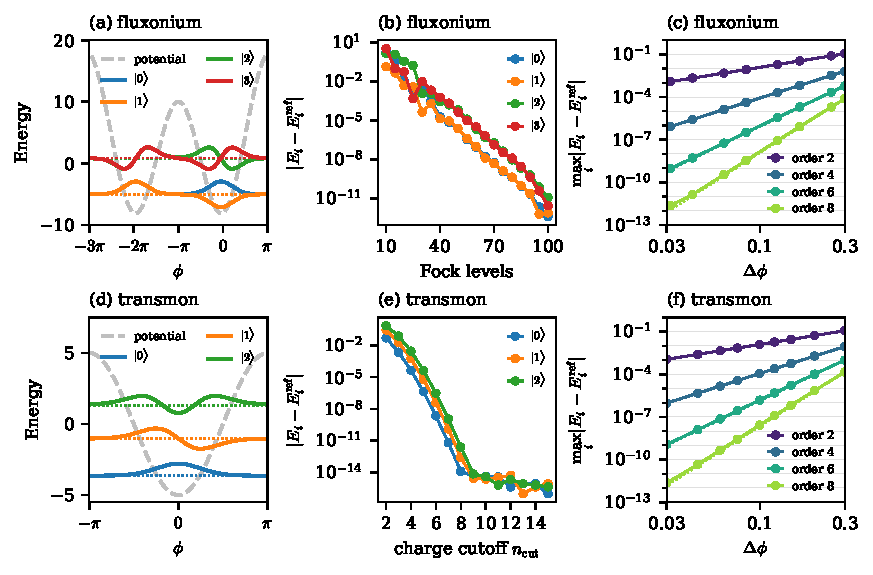
\includegraphics[width=\textwidth]{chapter-1-intro-background/figs/single_mode_convergence.pdf}
    \caption{Numerical diagonalization of a fluxonium (top) with $E_J=10$, $E_C=0.5$, $E_L=0.4$ and $\phi_{\rm ext}=\pi$, and a transmon (bottom) with $E_J=5$ and $E_C=0.2$.
    (a,d) Potential, lowest eigenvalues and wavefunctions in the phase basis, from \cref{lst:fluxonium_phase} ($201$ grid points) and \cref{lst:transmon_phase} ($160$ grid points, stencil of order $8$, $n_g=0$).
    (b) Error of the lowest four eigenvalues in the Fock basis versus the number of levels, relative to a $140$-level reference.
    (e) Error of the lowest three eigenvalues in the charge basis (\cref{lst:transmon_charge}) versus the charge cutoff $n_{\rm cut}$, relative to $n_{\rm cut}=40$, at $n_g=0.25$.
    (c,f) Largest eigenvalue error in the phase basis versus grid spacing, for finite-difference stencils of order $2$ to $8$ (\cref{lst:fluxonium_convergence}), with $n_g=0.25$ for the transmon.
    Dotted lines show $\Delta\phase^{p}$ for each order $p$.}
    \label{fig:single_mode_convergence}
\end{figure}

Similarly, for compact systems, we require a basis that spans possible $2\pi$ periodic wavefunctions.
The typical choice is the Fourier dual charge basis $\ket{\charge}$,
\begin{align}
         &\ket{\charge} 
         = 
         \frac {1}{\sqrt{2\pi}}
         \int_{-\pi}^{\pi} d\phase \,
         e^{i \charge  \phase} \ket{\phase} 
         , \quad \ket{\phase} 
         = 
         \frac {1}{\sqrt{2\pi}} 
         \sum_{\charge =-\infty}^\infty 
         e^{-i \charge  \phase} \ket{\charge}
         \, ,
\end{align}
which takes on integer values for each mode if coordinates are chosen as in \cref{sec:subtleties}.
In the charge basis, the charge operator $\charge$ is diagonal, and the  $\cos \phase$ operator is a sum of translations,
\begin{align}
e^{i  \hat \phase}
        = 
        \int d\phase \, e^{i \phase} \op{\phase}{\phase}
        = 
        \sum_{\charge =-\infty}^{\infty} \op{\charge  + 1}{\charge}  \, .
\end{align}

It is possible to use a $2\pi$ periodic phase basis directly.
Here the operators are qualitatively similar to the continuous case. The $\cos \phase$ operator is diagonal and the $\charge$ operator is a finite difference derivative.
The offset charge can enter in two equivalent ways.
One is to impose a twisted boundary condition $\psi(\phase + 2\pi) = e^{i 2\pi q} \psi(\phase)$ on the wavefunction, with a quasimomentum $q$.
Here the derivative wraps around with an additional phase depending on which side of the domain is being considered.
The other is to gauge the twist out of the wavefunction and into the Hamiltonian.
Writing $\psi(\phase) = e^{i q \phase} \chi(\phase)$, the function $\chi$ is $2\pi$ periodic, and the charge operator $\charge = -i\partial_\phase$ acts as $\charge \, \psi = -i \partial_\phase \left( e^{i q \phase} \chi \right) = e^{i q \phase} \left( \charge + q \right) \chi$.
A Hamiltonian $4 E_C (\charge - n_g)^2$ with twist $q$ is thus the periodic problem with offset charge $n_g - q$.
Here the finite difference derivative wraps around without any additional phases, and the whole offset charge appears explicitly in the Hamiltonian.

In \cref{lst:transmon_charge} and \cref{lst:transmon_phase} we show numpy code to diagonalize the transmon Hamiltonian $\hat H = 4 E_C (\hat\charge - n_g)^2 - E_J\cos(\hat\phase)$ in the charge and periodic phase bases.
The charge basis exhibits much faster convergence with the number of states included, and the phase basis solution is limited by the error of the finite difference derivative (\cref{fig:single_mode_convergence}).

An isolated transmon, fluxonium, or resonator is a single quantum mode, but we require methods to consider the multi-mode circuits quantized in the previous section.
As in standard quantum mechanics, we can combine two or more Hilbert spaces via a tensor product $\otimes$.
For example two systems $H_1$, $H_2$ can be represented by $H = H_{1} \otimes I + I \otimes H_2 + g_1\otimes g_2$, where $g_1\otimes g_2$ captures any coupling between the two systems.
The cost to naively represent a composite system grows with the product of the individual basis sizes.

A technique used to mitigate this cost is hierarchical diagonalization, which is available in scqubits \cite{groszkowskiScqubitsPythonPackage2021a,chittaComputeraidedQuantizationNumerical2022a}.
Rather than represent the full tensor product basis, each individual subsystem is diagonalized individually, and the coupling operator is then expressed in the eigenbases of the individual modes.
The full Hamiltonian is then
\begin{align}
  \label{eq:hierarchical_two_system}
  H = \textrm{diag}(E_0^{(1)}, E_1^{(1)}, \dots, E_{n-1}^{(1)}) \otimes I + I \otimes  \textrm{diag}(E_0^{(2)}, E_1^{(2)}, \dots, E_{m-1}^{(2)}) + V_1^\dagger g_1 V_1 \otimes V_2^\dagger g_2 V_2 \, ,
\end{align}
with $E_i^{(1)}$, $V_1$ and $E_i^{(2)}$, $V_2$ the eigenvalues and column-stacked eigenvector matrix of the 1st and 2nd system, respectively.
Rather than keep all eigenvalues/states, only the lowest $n$ and $m$ are kept.
The matrices $V_1$ and $V_2$ are thus rectangular with $n$ and $m$ columns, and the inverse is replaced by the conjugate transpose (the two are equivalent if all eigenvectors are kept).
The reduced size basis can still accurately represent lower energy dynamics in the composite system, although convergence must be studied on a case by case basis to ensure that enough states are being retained. 
\cref{lst:coupled_capacitive} implements hierarchical diagonalization for a capacitively coupled fluxonium and transmon.
\Citeauthor{kermanEfficientNumericalSimulation2020} \cite{kermanEfficientNumericalSimulation2020} provides a study on convergence and efficient hierarchical diagonalization techniques.


%=========================================================
\section{Mode-Preserving Coordinate Transformations} \label{sec:Transforms}
%=========================================================

The construction of \cref{sec:ModeTypes} fixes the retained coordinates only up to an invertible change of basis among the dynamical modes.
This section characterizes that freedom, identifies the compact block of the transformation as discrete, and poses the choice of basis as an optimization.
\Cref{sec:SymbolicSearch,sec:NumericalSearch} solves the problem both symbolically and numerically, illustrated by three tasks.

To characterize the remaining coordinate freedom, we ask which invertible transformation $S$ keeps the existing dynamical coordinates as compact, extended, and harmonic?
Following the index sets of \cref{sec:multicompact}, we write the transformation as a $3\times3$ block matrix, $S_{xy}$, with $x,y\in\{{\rm c},{\rm e},{\rm h}\}$.
Block multiplication gives the junction content of the new harmonic columns and the inductive content of the new compact columns,
\begin{align*}
    \bigl(\tilde\omega_J^TS\bigr)_{\rm h}&=\tilde\omega_{J,\rm c}^TS_{\rm ch}+\tilde\omega_{J,\rm e}^TS_{\rm eh} \, , \\
    \bigl(\tilde\omega_L^TS\bigr)_{\rm c}&=\tilde\omega_{L,\rm e}^TS_{\rm ec}+\tilde\omega_{L,\rm h}^TS_{\rm hc} \, .
\end{align*}
A harmonic coordinate must carry no junction term and a compact coordinate no inductive term, so both expressions must vanish.
This forces $S_{\rm ch}=S_{\rm eh}=0$ and $S_{\rm ec}=S_{\rm hc}=0$.
Extended coordinates already carry every term, so nothing restricts what they absorb.
The general type-preserving transformation is therefore
\begin{equation}
\begin{aligned}
    S&=\begin{pmatrix}S_{\rm cc}&S_{\rm ce}&0\\0&S_{\rm ee}&0\\0&S_{\rm he}&S_{\rm hh}\end{pmatrix}\,, \\
    S_{\rm relaxed}&=\begin{pmatrix}S_{\rm cc}&S_{\rm ce}&S_{\rm ch}\\0&S_{\rm ee}&S_{\rm eh}\\0&S_{\rm he}&S_{\rm hh}\end{pmatrix}\equiv\begin{pmatrix}S_{\rm cc}&S_{\rm cn}\\0&S_{\rm nn}\end{pmatrix} \, ,
\end{aligned}
\label{eq:S_structure}
\end{equation}
with rows and columns of $S$ ordered (compact, extended, harmonic).
Its determinant is $\det S_{\rm cc}\det S_{\rm ee}\det S_{\rm hh}$, so $S$ is invertible if and only if its three diagonal blocks are.
$S_{\rm relaxed}$ combines the extended and harmonic blocks into the noncompact block ${\rm n}={\rm e}\oplus{\rm h}$ and allows $S_{\rm ch},S_{\rm eh}\neq0$.
This still gives a valid set of coordinates, although it gives the harmonic coordinates junction content and relabels them extended.
This relabeling is innocuous, as extended and harmonic variables are both real valued variables.


\begin{figure}[t]
    \centering
    \resizebox{\linewidth}{!}{% Relaxing S_hc for the Fig. 1 transmon-resonator example: the compact phase varphi_1 and the
% harmonic resonator phase varphi_2 live on a cylinder. (a) The physical cylinder; (b) the strip
% cut open in sheared coordinates varphi_1 = varphi_u, varphi_2 = varphi_v + alpha varphi_u, whose edges are sewn
% with an offset; (c) the charges, where the integer transmon charge n_u - alpha n_v puts the
% allowed states on tilted lines and n_v stays continuous.
% Adapted from Notes/figs/compact_shear_cylinder.tex (panels a and c).
% Compile standalone with the draw-circuit driver; \input into main.tex via the standalone package.
\documentclass[border=9pt]{standalone}
\usepackage{amsmath,amssymb}
\usepackage{tikz}
\definecolor{figBlue}{RGB}{0,114,178}
\definecolor{figOrange}{RGB}{213,94,0}
\begin{document}
\begin{tikzpicture}[font=\small,>=latex,line cap=round,line join=round]
\node[font=\bfseries] at (1.7,6.2) {(a) Cylinder in $(\varphi_1,\varphi_2)$};
\begin{scope}[yshift=0.128cm,yscale=0.942]
\fill[black!3] (0.52,1) -- (0.52,5.2) arc[start angle=180,end angle=0,x radius=1.18,y radius=0.36] -- (2.88,1) arc[start angle=0,end angle=-180,x radius=1.18,y radius=0.36];
\draw[black!55] (0.52,1) -- (0.52,5.2) (2.88,1) -- (2.88,5.2);
\draw[black!55] (1.7,5.2) ellipse[x radius=1.18,y radius=0.36];
\draw[black!35,dashed] (2.88,1) arc[start angle=0,end angle=180,x radius=1.18,y radius=0.36];
\draw[black!55] (2.88,1) arc[start angle=0,end angle=-180,x radius=1.18,y radius=0.36];
\draw[black!40,dashed] (2.88,1) -- (2.88,5.2);
\draw[figBlue,line width=1.3pt,dashed] (2.88,2.9) arc[start angle=0,end angle=180,x radius=1.18,y radius=0.36];
\draw[figBlue,line width=1.3pt] (2.88,2.9) arc[start angle=0,end angle=-180,x radius=1.18,y radius=0.36];
\draw[figOrange,line width=1.2pt,dashed] plot[smooth] coordinates {(2.8800,2.9000) (2.8793,2.9209) (2.8771,2.9418) (2.8735,2.9626) (2.8685,2.9834) (2.8621,3.0042) (2.8542,3.0248) (2.8449,3.0454) (2.8343,3.0659) (2.8222,3.0862) (2.8088,3.1065) (2.7941,3.1265) (2.7780,3.1464) (2.7606,3.1661) (2.7419,3.1857) (2.7219,3.2050) (2.7007,3.2241) (2.6783,3.2430) (2.6546,3.2616) (2.6299,3.2800) (2.6039,3.2981) (2.5769,3.3159) (2.5488,3.3334) (2.5197,3.3506) (2.4896,3.3675) (2.4585,3.3841) (2.4265,3.4004) (2.3936,3.4162) (2.3598,3.4318) (2.3253,3.4470) (2.2900,3.4618) (2.2540,3.4762) (2.2173,3.4902) (2.1799,3.5039) (2.1420,3.5171) (2.1036,3.5300) (2.0646,3.5424) (2.0253,3.5544) (1.9855,3.5660) (1.9453,3.5771) (1.9049,3.5879) (1.8642,3.5982) (1.8233,3.6080) (1.7823,3.6175) (1.7412,3.6264) (1.7000,3.6350) (1.6588,3.6431) (1.6177,3.6508) (1.5767,3.6580) (1.5358,3.6648) (1.4951,3.6712) (1.4547,3.6771) (1.4145,3.6826) (1.3747,3.6877) (1.3354,3.6924) (1.2964,3.6966) (1.2580,3.7005) (1.2201,3.7039) (1.1827,3.7069) (1.1460,3.7095) (1.1100,3.7118) (1.0747,3.7136) (1.0402,3.7151) (1.0064,3.7162) (0.9735,3.7170) (0.9415,3.7174) (0.9104,3.7175) (0.8803,3.7173) (0.8512,3.7167) (0.8231,3.7159) (0.7961,3.7147) (0.7701,3.7133) (0.7454,3.7116) (0.7217,3.7096) (0.6993,3.7074) (0.6781,3.7050) (0.6581,3.7023) (0.6394,3.6995) (0.6220,3.6964) (0.6059,3.6932) (0.5912,3.6898) (0.5778,3.6862) (0.5657,3.6826) (0.5551,3.6788) (0.5458,3.6748) (0.5379,3.6708) (0.5315,3.6668) (0.5265,3.6626) (0.5229,3.6584) (0.5207,3.6542) (0.5200,3.6500)};
\draw[figOrange,line width=1.2pt] plot[smooth] coordinates {(0.5200,3.6500) (0.5207,3.6458) (0.5229,3.6416) (0.5265,3.6374) (0.5315,3.6332) (0.5379,3.6292) (0.5458,3.6252) (0.5551,3.6212) (0.5657,3.6174) (0.5778,3.6138) (0.5912,3.6102) (0.6059,3.6068) (0.6220,3.6036) (0.6394,3.6005) (0.6581,3.5977) (0.6781,3.5950) (0.6993,3.5926) (0.7217,3.5904) (0.7454,3.5884) (0.7701,3.5867) (0.7961,3.5853) (0.8231,3.5841) (0.8512,3.5833) (0.8803,3.5827) (0.9104,3.5825) (0.9415,3.5826) (0.9735,3.5830) (1.0064,3.5838) (1.0402,3.5849) (1.0747,3.5864) (1.1100,3.5882) (1.1460,3.5905) (1.1827,3.5931) (1.2201,3.5961) (1.2580,3.5995) (1.2964,3.6034) (1.3354,3.6076) (1.3747,3.6123) (1.4145,3.6174) (1.4547,3.6229) (1.4951,3.6288) (1.5358,3.6352) (1.5767,3.6420) (1.6177,3.6492) (1.6588,3.6569) (1.7000,3.6650) (1.7412,3.6736) (1.7823,3.6825) (1.8233,3.6920) (1.8642,3.7018) (1.9049,3.7121) (1.9453,3.7229) (1.9855,3.7340) (2.0253,3.7456) (2.0646,3.7576) (2.1036,3.7700) (2.1420,3.7829) (2.1799,3.7961) (2.2173,3.8098) (2.2540,3.8238) (2.2900,3.8382) (2.3253,3.8530) (2.3598,3.8682) (2.3936,3.8838) (2.4265,3.8996) (2.4585,3.9159) (2.4896,3.9325) (2.5197,3.9494) (2.5488,3.9666) (2.5769,3.9841) (2.6039,4.0019) (2.6299,4.0200) (2.6546,4.0384) (2.6783,4.0570) (2.7007,4.0759) (2.7219,4.0950) (2.7419,4.1143) (2.7606,4.1339) (2.7780,4.1536) (2.7941,4.1735) (2.8088,4.1935) (2.8222,4.2138) (2.8343,4.2341) (2.8449,4.2546) (2.8542,4.2752) (2.8621,4.2958) (2.8685,4.3166) (2.8735,4.3374) (2.8771,4.3582) (2.8793,4.3791) (2.8800,4.4000)};
\fill[figBlue] (2.88,2.9) circle(2.5pt);
\node[right=4pt] at (2.88,2.9) {$(0,0)$};
\fill[figOrange] (2.88,4.4) circle(2.5pt);
\node[right=4pt] at (2.88,4.4) {$(0,2\pi\alpha)$};
\draw[<->,black!65] (-0.12,0.7) -- (-0.12,5.640) node[above] {$\varphi_2\in\mathbb R$};
\draw[->,black!65] (2.7,0.5) arc[start angle=30,end angle=-170,x radius=1.15,y radius=0.24];
\node at (1.7,-0.242) {$\varphi_1\in(0,2\pi]$};
\end{scope}
\begin{scope}[xshift=6.0cm]
% (b) strip at half height
\node[font=\bfseries] at (1.65,6.2) {(b) Cut open in $(\varphi_u,\varphi_v)$};
\fill[black!3] (0,3.55) rectangle (3.3,5.45);
\draw[<->,black!65] (0,3.45) -- (0,5.6);
\draw[<->,black!65] (3.3,3.45) -- (3.3,5.6);
\node[above,inner sep=1pt] at (0,5.6) {$\varphi_v$};
\node[above,inner sep=1pt] at (3.3,5.6) {$\varphi_v$};
\draw[->,figOrange,line width=1.2pt] (0,4.55) -- (3.25,4.55);
\node[above=2pt,font=\footnotesize] at (1.65,4.55) {fixed $\varphi_v$};
\draw[->,figBlue,line width=1.3pt] (0,4.55) -- (3.25,3.762);
\node[below=1pt,rotate=-13.6,font=\footnotesize] at (1.4,4.21) {fixed $\varphi_2$};
\fill[figBlue] (0,4.55) circle(2.5pt) (3.3,3.75) circle(2.5pt);
\fill[figOrange] (3.3,4.55) circle(2.5pt);
\node[left=4pt] at (0,4.55) {$(0,0)$};
\node[right=4pt] at (3.3,3.75) {$(2\pi,-2\pi\alpha)$};
\node[right=4pt] at (3.3,4.55) {$(2\pi,0)$};
\draw[->,black!65] (0,3.15) -- (3.3,3.15) node[right] {$\varphi_u$};
\node[below=2pt] at (0,3.15) {$0$};
\node[below=2pt] at (3.3,3.15) {$2\pi$};
% (c) charge plane: allowed states n_1 = n_u - alpha n_v in Z (blue); n_v stays continuous
\node[font=\bfseries] at (1.65,2.35) {(c) Charges in $(n_v,n_u)$};
\fill[black!3] (0,-0.15) rectangle (3.3,1.75);
\draw[->,black!65] (-0.1,0.8) -- (3.45,0.8) node[right,inner sep=2pt] {$n_v$};
\draw[->,black!65] (1.65,-0.25) -- (1.65,1.9) node[right,inner sep=2pt] {$n_u$};
\begin{scope}
\clip (0,-0.15) rectangle (3.3,1.75);
\foreach \m in {-3,...,3} {
  \draw[figBlue,line width=1.3pt] (0,0.8+0.6*\m-0.495) -- (3.3,0.8+0.6*\m+0.495);
}
\end{scope}
\node[right,figBlue,font=\footnotesize] at (3.3,1.45) {$n_u-\alpha n_v\in\mathbb Z$};
\end{scope}
\node[align=center,font=\normalsize] at (4.7,-0.95) {$\varphi_1=\varphi_u,\qquad \varphi_2=\varphi_v+\alpha \varphi_u,\qquad
\psi(\varphi_u,\varphi_v)=\psi(\varphi_u+2\pi,\varphi_v-2\pi\alpha)$};
\end{tikzpicture}
\end{document}
}
    \caption{{\bf $S_{\rm hc}$ twists the compact boundary condition.}
    For the circuit of \cref{fig:example_circuit}, the transmon phase $\varphi_1$ is periodic and the resonator phase $\varphi_2$ is real, so the configuration space is a cylinder (a).
    The blue path makes one turn at fixed $\varphi_2$ and closes at $(0,0)$.
    In the coordinates $\varphi_1=\varphi_u$, $\varphi_2=\varphi_v+\alpha\varphi_u$ (b), a turn at fixed $\varphi_v$ (orange) ends at the distinct point $(2\pi,0)$, which is $(0,2\pi\alpha)$ on the cylinder.
    (c) The transmon's integer charge is $n_u-\alpha n_v$, so the allowed charges lie on tilted lines while $n_v$ remains continuous.}
    \label{fig:compact_shear}
\end{figure}

The compact block columns are more restricted, and \cref{fig:compact_shear} shows what can go wrong by relaxing the zeros in the first column.
Consider $S_{\rm hc}=\alpha$ for the example of \cref{fig:example_circuit}.
This gives the transformed inductive incidence matrix $\tilde\omega_L^TS=\begin{pmatrix}\alpha&1\end{pmatrix}$, which has inductive content in the compact column.
The new coordinates follow from $S^{-1}$ and their conjugate momenta from $S^T$,
\begin{align*}
    \begin{pmatrix}\varphi_u\\\varphi_v\end{pmatrix}&=\begin{pmatrix}1&0\\-\alpha&1\end{pmatrix}\begin{pmatrix}\varphi_1\\\varphi_2\end{pmatrix}\,,\,\,
    \begin{pmatrix}n_u\\n_v\end{pmatrix}=\begin{pmatrix}1&\alpha\\0&1\end{pmatrix}\begin{pmatrix}n_1\\n_2\end{pmatrix}\,,
\end{align*}
so $\varphi_u$ enters the inductive energy of $L_r$ through $\varphi_2=\varphi_v+\alpha\varphi_u$.
The periodic boundary condition becomes $\psi(\varphi_u,\varphi_v)=\psi(\varphi_u+2\pi,\varphi_v-2\pi\alpha)$, and the quantized charge of the compact mode sits in $n_1=n_u-\alpha n_v$.
Like in \cref{sec:multicompact}, the variable $\varphi_u$ cannot be treated as an independent rotor.
Such coordinates can still be quantized with careful bookkeeping, but $\mathcal A$ excludes them so that \cref{eq:compact_bc} continues to hold axis by axis.
The remaining entry of the compact column, $S_{cc}$, corresponds to a different choice of linearly independent rows in \cref{eq:reference_compact}, so $S_{cc}$ has a set of discrete choices.

The admissible set of transformations $\mathcal{A}$ therefore consists of \cref{eq:S_structure}, with $S_{\rm cc}\in\bigl(\tilde\omega_{J,\mathcal K}^T\bigr)^{-1}$ derived from a linearly independent set of rows $\mathcal{K}$ and $S_{\rm ee}$, $S_{\rm hh}$ invertible.
The set $\mathcal{A}_{\rm relaxed}$ is the same with $S_{\rm ch}$ and $S_{\rm eh}$ free.

We now frame the specific choice of $S$ as an optimization.
We aim to identify an optimal $S^\star \in \mathcal{A}$ or $\mathcal{A_{\rm relaxed}}$ that minimizes a cost $\costFunc$
\begin{align}
    S^\star=\arg\min_{S\in\mathcal A}\ \costFunc\bigl(\mathcal H_S;\ \lambda\bigr) \, ,
    \label{eq:opt_problem}
\end{align}
where $\mathcal H_S$ is the Hamiltonian in the coordinates defined by $S$, parametrized by circuit parameters $\lambda$.
It depends on $S$ through $S^T\tilde CS$, $S^T\tilde L^*S$, and $\tilde\omega_J^TS$, together with the transformed offsets $S^T\tilde Q_g$ and $S^T\tilde\omega_L L_b^{-1}\B_L\Phi_{\rm ext}$.
A cost may act on these matrices directly, or on quantities that require solving for the states of $\mathcal H_S$.
The accompanying code~\cite{weissler2026circuitquantizationcode} takes $\costFunc$ as a user-supplied function.
The two routes below differ in whether $\lambda$ is kept symbolic and parameter independent.

\subsection{Parameter-Independent Symbolic Search}\label{sec:SymbolicSearch}

The first route keeps the circuit parameters $\lambda = \{C_k, L_k, E_{J,k}, n_g, \PhiExt\}$ symbolic and seeks a coordinate transformation $S^\star \in \mathcal{A}$ (or $\mathcal{A}_{\rm relaxed}$) whose entries are rational numbers independent of $\lambda$.
The dynamical coordinates are then fixed by the circuit topology alone.

Every element of the transformed circuit matrices is a polynomial in the transformation entries and circuit parameters, which limits what can be solved.
The only conditions that hold irrespective of circuit parameters must exclusively constrain the transformation entries.
We represent these conditions as a set of polynomial equalities $\targets$, for which any given $S$ fulfills a subset $\targetSubset(S) \subseteq \targets$.
The symbolic route solves \cref{eq:opt_problem} for any cost of the form $\costFunc\bigl(\targetSubset(S)\bigr)$, which depends on the subset of conditions fulfilled.
Because there are finitely many choices for the compact block $S_{\rm cc}$ (\cref{eq:reference_compact}), we iterate over each option and search the remaining blocks.

For a fixed $S_{\rm cc}$, a condition requires some expression $E(\mathbf{s},\lambda)$ to vanish for all $\lambda$, where $E$ is built from $S$ and the circuit matrices by products and inverses, such as an entry of $(S^T\tilde{C}S)^{-1}$ or of the junction matrix.
Such an expression is a rational function of the unknown entries $\mathbf{s}$ of the remaining blocks and of $\lambda$.
Clearing denominators and expanding the numerator in monomials of the circuit parameters, $\text{num}(E) = \sum_{\alpha} f_{E,\alpha}(\mathbf{s}) \lambda^{\alpha}$ vanishes for all $\lambda$ exactly when every coefficient $f_{E,\alpha}(\mathbf{s})$ does.
We therefore allow in $\targets$ any condition that reduces to a polynomial system in $\mathbf{s}$ alone.

A pattern $\pattern \subseteq \targets$ is feasible when its systems have a common solution, and we structure a search to find the highest scoring pattern.
Candidate patterns are considered in non-decreasing order of $\costFunc$, skipping any that contain a subset already found to be infeasible.
The search stops at the first level where a feasible solution is found.

The solutions of a feasible pattern generally form under-constrained systems of polynomials, which we solve using algebraic geometry techniques.
Using \texttt{Singular}~\cite{Singular_2024}, we decompose each into irreducible components and compute its Gr\"obner cover~\cite{montes_wibmer_groebner_cover_2010}, which parameterizes every valid transformation by a maximal independent set of free entries $\mathbf{s}_{\rm free}$.
The remaining entries are rational functions of them.
Every choice of $\mathbf{s}_{\rm free}$ fulfills the same pattern and obtains the same cost.
Any ties under $\costFunc$, or decisions on free entries, are left to the task.
\Cref{sec:Enumeration} fixes both for the case of circuit enumeration.

\subsubsection{Application: Hamiltonian classes for circuit enumeration}\label{sec:Enumeration}

As an example of the symbolic search, we consider circuit enumeration, or generating every distinct circuit built from a fixed set of elements, such as capacitors, inductors, and Josephson junctions.
In Ref.~\cite{weissler2026enumerationsuperconductingcircuits5}, we cataloged these circuits by writing down one representative set of coordinates per circuit, chosen by the same rule for every circuit, so that the Hamiltonians of different circuits could be compared directly.
The functional form of the resulting Hamiltonian, with the parameter values stripped, served as a ``Hamiltonian class.''
Here we place that procedure concretely within the admissible set $\mathcal{A}$, as the minimizer of a pattern cost.

The cost is a two stage procedure that seeks to minimize intermode coupling.
The targets of the first stage are the off-diagonal entries of the junction matrix $\sum_k E_{J,k} (\tilde{\omega}_{J,k}^T S)^T (\tilde{\omega}_{J,k}^T S)$, which are nonzero exactly when any junction phase involves both modes.
This stage maximizes the number of vanishing entries.
The second stage takes the off-diagonal entries of $S^T \tilde{L}^* S$ and $(S^T \tilde{C} S)^{-1}$ and again maximizes the number of zero entries, subject to the constraints imposed by the first stage.
Among ties, fewer inductive couplings are chosen.

The winning family still has free entries $\mathbf{s}_{\rm free}$, which the pattern cost cannot see.
They set the phase arguments of the extended modes, so they must be fixed the same way for every circuit to give a consistent class label.
We fix them by a second, discrete optimization that requires integer junction coefficients on the extended columns (e.g., $\cos(2\varphi)$ rather than $\cos(1.45\varphi)$) and minimizes their $\ell_1$ norm.
We solve this optimization using the \texttt{Z3} SMT solver~\cite{DeMouraBjornerZ3_2008} to obtain a provably optimal answer.
Free parameters absent from $\tilde{\omega}_J^T S$, such as harmonic scalings in $S_{\rm hh}$, take the simplest rational values that leave $S$ invertible, yielding a concrete $S^\star$.

\begin{figure}[t]
    \centering
    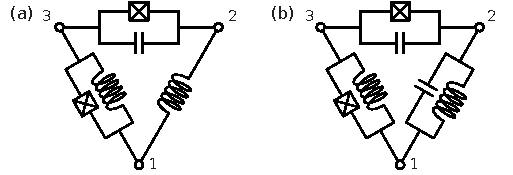
\includegraphics[width=\linewidth]{chapter-2-quantization/figs/diff_class_example.pdf}
    \caption{{\bf The Hamiltonian class depends on the cost.}
    Circuit (b) adds a capacitor $C_{12}$ in parallel with the inductor between nodes 1 and 2 of circuit (a).
    Adapted from Ref.~\cite{weissler2026enumerationsuperconductingcircuits5}.}
    \label{fig:diff_class_example}
\end{figure}

As a worked example, consider the circuits of \cref{fig:diff_class_example}, with node 3 as reference and node coordinates $\Phi_1-\Phi_3$ and $\Phi_2-\Phi_3$.
Both coordinates are extended, so any invertible $S=\bigl(\begin{smallmatrix}a&b\\c&d\end{smallmatrix}\bigr)$ is admissible.
Each junction acts on a single node coordinate, so $\tilde\omega_J^TS=S$ and the off-diagonal entry of the junction matrix is $E_{J,31}\,ab+E_{J,32}\,cd$.
It vanishes for all parameters exactly when $ab=cd=0$.
The second-stage targets multiply out to
\begin{align*}
    \bigl(S^T\tilde L^*S\bigr)_{12}&=\frac{ab}{L_{31}}+\frac{(a-c)(b-d)}{L_{21}} \, , \\
    \bigl(S^T\tilde CS\bigr)_{12}&=C_{31}\,ab+C_{32}\,cd+C_{12}\,(a-c)(b-d) \, ,
\end{align*}
where $C_{31}$ and $C_{32}$ include the junction capacitances and $C_{12}=0$ in circuit (a).
With two modes, the off-diagonal entry of $(S^T\tilde CS)^{-1}$ is proportional to $(S^T\tilde CS)_{12}$, so both give the same target.
Collecting the coefficient of each parameter, inductive decoupling requires $ab=0$ and $(a-c)(b-d)=0$, while charge decoupling requires $ab=cd=0$, together with $(a-c)(b-d)=0$ in circuit (b).
The first stage fixes $ab=cd=0$, so $S$ is diagonal up to a swap of columns and keeps the node coordinates.
The inductive entry is then $-ad/L_{21}\neq0$, while the charge entry $-ad\,C_{12}$ vanishes only in circuit (a).
The resulting classes are $q_1^2+q_2^2+\varphi_1^2+\varphi_1\varphi_2+\varphi_2^2+\cos\varphi_1+\cos\varphi_2$ for (a), with an additional $q_1q_2$ for (b).
Inductive decoupling instead forces $b=0$ and $c=a$, which places junction 32 on both coordinates, so the two patterns are mutually exclusive.
A cost that ranks the inductive entry first selects this family, and the integer-coefficient step sets $a=1$ and $d=\pm1$, and with $d=-1$ the second coordinate is $\Phi_1-\Phi_2$.
Both circuits then fall into the same class, $q_1^2+q_1q_2+q_2^2+\varphi_1^2+\varphi_2^2+\cos(\varphi_1-\varphi_2)+\cos\varphi_1$, trading the linear coupling $\varphi_1\varphi_2$ for a nonlinear one.

\subsection{Numerical Search}\label{sec:NumericalSearch}

The symbolic route sees only conditions that hold for every parameter value, but transformations that depend on circuit parameter values can be very useful.
For such tasks we can fix $\lambda$ at numerical values and minimize $\costFunc$ over the continuous blocks of $S$ for each discrete choice of the compact block.

To optimize over invertible matrices, we use the polar decomposition to parametrize $\mathcal{A}$ with unconstrained real variables \cite{horn2013matrix,gallier2020differential} .
The polar decomposition writes any real invertible matrix $D$ as $D=QP$, with $Q$ orthogonal and $P$ symmetric positive definite.
Each factor is the exponential of a simpler matrix.
Any symmetric positive-definite $P = e^{B}$ for a unique symmetric $B$, and any orthogonal $Q$ with $\det Q=+1$ equals $e^{A}$ for some antisymmetric $A$.
Every $D$ with $\det D>0$ can therefore be written as $D=e^{A}e^{B}$, and negative determinants can be reached by flipping the sign of a column.
Antisymmetry forces the diagonal of $A$ to vanish, so the free entries are those of $A$ above the diagonal and of $B$ on and above it.
For each discrete choice of $S_{\rm cc}$, we thus substitute
\begin{align}
S_{\rm ee}=e^{A_{\rm ee}}e^{B_{\rm ee}},\; S_{\rm hh}=e^{A_{\rm hh}}e^{B_{\rm hh}},\; S_{\rm nn}=e^{A_{\rm nn}}e^{B_{\rm nn}}
\label{eq:S_numerical}
\end{align}
into \cref{eq:S_structure} and leave the remaining blocks other than $S_{\rm cc}$ unconstrained.
The optimization is then over the independent entries of $(A_{\rm ee},B_{\rm ee},A_{\rm hh},B_{\rm hh},S_{\rm ce},S_{\rm he})$ for $\mathcal{A}$, or of $(A_{\rm nn},B_{\rm nn},S_{\rm cn})$ for $\mathcal{A}_{\rm relaxed}$.
Any cost $\costFunc$ that returns a real scalar can be used, and it can be minimized with any standard optimization routine.

One thing to be aware of is that coordinates found by the numerical search depend on the circuit parameters, so they require care when those parameters change in time.
As for a standard rotating frame, the unitary $U(t)$ implementing it adds the generator term $-i\hbar\,U^\dagger(t)\,\partial_tU(t)$ to the transformed Hamiltonian, which must be kept or avoided by fixing $S^\star$ at a single operating point.
The irrotational assignment of \cref{sec:tdflux} is an instance of the same construction.
Changing $\B$ is a time-dependent translation of the node fluxes, and the irrotational choice is the one whose generator term cancels the explicit $\dot\Phi_{\rm ext}$ dependence of the offset charge.

As a concrete example, consider normal mode diagonalization based on Williamson's theorem \cite{Williamson1936NormalForms},
which has been widely used in superconducting circuits to identify coordinates that remove all quadratic coupling in the Hamiltonian \cite{niggBlackBoxSuperconductingCircuit2012, smithQuantizationInductivelyShunted2016,royMultimodeSuperconductingCircuits2018, gelyQuCATQuantumCircuit2020,kermanEfficientNumericalSimulation2020, ding_free-mode_2021,rasmussenSuperconductingCircuitCompanionan2021, Egusquiza_Algebraic_2022, rajabzadehAnalysisArbitrarySuperconducting2023, smitham2024reciprocallumpedelementsuperconductingcircuits}.
We can express the transformation as the minimum of a cost on the residual coordinate freedom.
For $C'=S^T\tilde C S$ and $L'=S^T\tilde L^*S$, the normal mode transformation is the minimum of
\begin{align}
\costFunc_{\rm NM}(S)
=\sum_{\substack{i<j\\j\not\subset{\rm c}}}
\left(C'_{ij}\right)^2
+\sum_{\substack{i<j\\\{i,j\}\in{\rm n}}}
\left(L'_{ij}\right)^2 .
\label{eq:numerical_normal_cost}
\end{align}
The first sum omits the compact column blocks, and the second sum considers only the non-compact modes.

Of course, this solution can also be obtained analytically.
In compact/noncompact blocks, choose $S_{\rm cn}=-\tilde C_{\rm cc}^{-1}\tilde C_{\rm cn}S_{\rm nn}$ to remove any charge coupling between the compact and non-compact modes.
In other words, this shear sets $[S^T \tilde CS]_{\rm ce}=[S^T \tilde CS]_{\rm ch}=0$.
The retained noncompact block of $S^T\tilde CS$ is then $S_{\rm nn}^T\bar C_{\rm nn}S_{\rm nn}$, with the Schur complement $\bar C_{\rm nn}=\tilde C_{\rm nn}-\tilde C_{\rm nc}\tilde C_{\rm cc}^{-1}\tilde C_{\rm cn}$.
For the remaining noncompact block, $S_{\rm nn}$, choose the columns to solve the eigenvalue problem $\bar C_{\rm nn}^{-1}\tilde L^*_{\rm nn}v_i=\lambda_iv_i$.
Because $S_{\rm ch}$ and $S_{\rm eh}$ are nonzero, normal modes fall in the relaxed family of transformations.
If the basis is chosen to be $\bar C_{\rm nn}$-orthonormal, then both sums vanish.
Conversely, a transformation satisfying $\costFunc_{\rm NM}(S)=0$ simultaneously diagonalizes the two noncompact quadratic forms, so its columns solve the generalized eigenvalue problem $\tilde L^*_{\rm nn}v_i=\lambda_i\bar C_{\rm nn}v_i$.

\begin{figure}[t]
    \centering
    % The 0-pi qubit (Brooks, Kitaev, Preskill; Dempster et al.; Groszkowski et al.) (a), and the
% four columns of its mode basis Z (b)-(e), in the style of lclc_box_modes.tex.
% Ring J1 (1-2), L1 (2-3), J2 (3-4), L2 (4-1), threaded by Phi_ext, with C1 (1-3) and C2 (2-4)
% across the diagonals, which cross at the center without connecting (C2 hops over C1).
% Node numbering matches Groszkowski et al. Eq. (1) and the text of Sec. III.C.
% In (b)-(e) each node carries the sign of its entry in that column of Z (main.tex, 0-pi paragraph);
% branches whose flux vanishes in that column are grey.
% Compile standalone with the draw-circuit driver; \input into main.tex.
% The josephson bipole comes from jj_bipoles.tex, which main.tex also loads.
\documentclass[border=8pt]{standalone}
\usepackage{tikz}
\usepackage{circuitikz}
\input{jj_bipoles}
\begin{document}
\begin{circuitikz}[line width=0.8pt, font=\small]
    \ctikzset{label/align = straight, bipoles/thickness=1, capacitors/scale=0.55, inductors/scale=0.9, inductors/coils=4, misc/scale=0.8}
    \tikzset{
        nd/.style={circle, fill, inner sep=1.1pt},
        off/.style={color=black!30},
        sgn/.style={font=\scriptsize, inner sep=1pt},
        panelcap/.style={font=\footnotesize, align=center},
    }

    % (a) the circuit: square of side 2.8, flat side down
    \coordinate (n1) at (0,2.8);
    \coordinate (n2) at (2.8,2.8);
    \coordinate (n3) at (2.8,0);
    \coordinate (n4) at (0,0);
    \coordinate (c) at (1.4,1.4);
    \draw (n1) to[josephson, l=$J_1$] (n2);
    \draw (n2) to[L, l=$L_1$] (n3);
    \draw (n3) to[josephson, l=$J_2$] (n4);
    \draw (n4) to[L, l=$L_2$] (n1);
    \draw (n1) -- (0.3,2.5) to[C] (0.9,1.9) -- (n3);
    \draw (n2) -- (2.5,2.5) to[C] (1.9,1.9) -- ([shift={(45:0.13)}]c) arc[start angle=45, end angle=225, radius=0.13] -- (n4);
    \foreach \n in {n1,n2,n3,n4} {\node[nd] at (\n) {};}
    \node at (1.1,2.1) {$C_1$};
    \node at (1.7,2.1) {$C_2$};
    \node[above left] at (n1) {1};
    \node[above right] at (n2) {2};
    \node[below right] at (n3) {3};
    \node[below left] at (n4) {4};
    \node at (1.4,0.55) {$\odot\,\Phi_{\rm ext}$};
    \node[panelcap] at (1.4,-0.95) {(a) 0-$\pi$ qubit};

    % (b)-(e) the columns of Z: node signs, and grey branches with zero flux.
    % #1 x, #2 y, #3..#6 signs at nodes 1..4, #7 J style, #8 L style, #9 C style
    \newcommand{\zppanel}[9]{
        \begin{scope}[shift={(#1,#2)}]
            \ctikzset{capacitors/scale=0.32, inductors/scale=0.5, misc/scale=0.5}
            \draw[#7] (0,1.1) to[josephson] (1.1,1.1);
            \draw[#7] (1.1,0) to[josephson] (0,0);
            \draw[#8] (1.1,1.1) to[L] (1.1,0);
            \draw[#8] (0,0) to[L] (0,1.1);
            \draw[#9] (0,1.1) -- (0.15,0.95) to[C] (0.43,0.67) -- (1.1,0);
            \draw[#9] (1.1,1.1) -- (0.95,0.95) to[C] (0.67,0.67) -- ([shift={(45:0.07)}]0.55,0.55) arc[start angle=45, end angle=225, radius=0.07] -- (0,0);
            \foreach \x/\y in {0/1.1, 1.1/1.1, 1.1/0, 0/0} {\node[nd] at (\x,\y) {};}
            \node[sgn, above left] at (0,1.1) {$#3$};
            \node[sgn, above right] at (1.1,1.1) {$#4$};
            \node[sgn, below right] at (1.1,0) {$#5$};
            \node[sgn, below left] at (0,0) {$#6$};
        \end{scope}
    }
    \zppanel{4.0}{1.65}{+}{-}{-}{+}{}{off}{}
    \node[panelcap] at (4.55,1.1) {(b) compact};
    \zppanel{5.9}{1.65}{+}{-}{+}{-}{}{}{off}
    \node[panelcap] at (6.45,1.1) {(c) extended};
    \zppanel{4.0}{-0.55}{+}{+}{-}{-}{off}{}{}
    \node[panelcap] at (4.55,-1.1) {(d) harmonic};
    \zppanel{5.9}{-0.55}{+}{+}{+}{+}{off}{off}{off}
    \node[panelcap] at (6.45,-1.1) {(e) cyclic};
\end{circuitikz}
\end{document}

    \caption{{\bf Mode types of the 0-$\pi$ qubit}~\cite{brooks2013,Dempster2014understanding,groszkowski2018}.
    (a) The circuit, with nodes 1--4.
    The diagonals carrying $C_1$ and $C_2$ cross without connecting.
    (b)--(e) The columns of $\trans$ in \cref{sec:NumericalSearch}, with the sign of each node's entry.
    Grey branches carry no flux difference in that column, so they contribute no energy.}
    \label{fig:zeropi}
\end{figure}

The 0-$\pi$ qubit~\cite{brooks2013,Dempster2014understanding,groszkowski2018} shows when the normal modes leave $\mathcal A$.
Its circuit (\cref{fig:zeropi}) alternates the junctions $J_1$ (nodes 1--2) and $J_2$ (3--4) with the inductors $L_1$ (2--3) and $L_2$ (4--1), and the capacitors $C_1$ and $C_2$ join the opposite nodes 1--3 and 2--4.
The null spaces give one compact, one extended, one harmonic, and one cyclic mode,
\begin{align*}
    Z=\begin{pmatrix}
       \phantom{-}1 &\phantom{-}1 &\phantom{-}1 &\phantom{-}1\\
        -1 & -1 &\phantom{-}1 &\phantom{-}1\\
        -1 &\phantom{-}1 & -1 &\phantom{-}1\\
       \phantom{-}1 & -1 & -1 &\phantom{-}1
    \end{pmatrix},
\end{align*}
with columns in this order depicted in \cref{fig:zeropi} (b)--(e).
The standard coordinates $(\theta,\phi,\zeta)$ of Refs.~\cite{Dempster2014understanding,groszkowski2018} follow from $S={\rm diag}(-\tfrac12,-\tfrac12,\tfrac12)$, which lies in $\mathcal A$.
In them, the junction phases are $\phi\pm\theta$, the inductor phases $\phi\pm\zeta$, and the capacitor phases $\theta\pm\zeta$.
With identical elements, the cross terms cancel within each pair, so $\tilde C$ and $\tilde L^*$ are diagonal and $(\theta,\phi,\zeta)$ are the normal modes.

Disorder breaks this cancellation pair by pair.
With the relative deviations $dX=(X_1-X_2)/X$ of Ref.~\cite{groszkowski2018}, $dC_J$ couples $\theta$ and $\phi$ through $\tilde C$, $dC$ couples $\theta$ and $\zeta$ through $\tilde C$, and $dE_L$ couples $\phi$ and $\zeta$ through $\tilde L^*$, while $dE_J$ enters neither quadratic form.
To first order in the disorder, the normal modes follow from $(\theta,\phi,\zeta)$ by
\begin{align*}
    S=\begin{pmatrix}
        1 & -\frac{C_J\,dC_J}{2(C+C_J)} & \frac{C\,dC}{2(C+C_J)}\\
        0 & 1 & -\frac{C\,dE_L}{2(C-C_J)}\\
        0 & \frac{C_J\,dE_L}{2(C-C_J)} & 1
    \end{pmatrix} \, ,
\end{align*}
which lies in $\mathcal A_{\rm relaxed}$ if $dC$ or $dE_L$ are nonzero.
The normal-mode $\zeta$ thus enters both junctions with a weight on the order of the disorder, so the coupling moves from the quadratic terms into the cosines.

\subsubsection{Application: product-state coordinates}

\begin{figure}[t]
    \centering
    \begin{minipage}[t]{0.47\columnwidth}
        \raggedright{\small (a)}\par\vspace{2pt}
        \resizebox{\linewidth}{!}{% The cos(2 phi) transmon (KITE) of Roverch et al., drawn as in the source: a
% hexagonal loop with a junction on each vertical side and an inductor on each diagonal,
% threaded by Phi_ext, shunted by C_S between the top node and ground. Only the
% shunted node carries capacitance to ground, so the two modes in which a junction's
% terminals move together are frozen. Reference frame: varphi (compact, across C_S),
% phi_Sigma and phi_Delta (sum and difference of the two upper inductor phases).
% Compile standalone with the draw-circuit driver; \input into main.tex via the
% standalone package. The josephson bipole comes from jj_bipoles.tex, which main.tex also loads.
\documentclass[border=3pt]{standalone}
\usepackage{tikz}
\usepackage{circuitikz}
\input{jj_bipoles}
\begin{document}
\begin{circuitikz}[line width=0.7pt, font=\small]
    \ctikzset{label/align = straight, bipoles/thickness=1, capacitors/scale=0.55, inductors/scale=0.9, inductors/coils=4, misc/scale=0.8}
    \tikzset{lbl/.style={font=\small, inner sep=0.5pt}}
    \coordinate (T) at (0,1.7);
    \coordinate (B) at (0,-1.7);
    \coordinate (UL) at (-1.472,0.85);
    \coordinate (LL) at (-1.472,-0.85);
    \coordinate (UR) at (1.472,0.85);
    \coordinate (LR) at (1.472,-0.85);
    \coordinate (CT) at (-2.2,1.7);
    \coordinate (CB) at (-2.2,-1.7);
    % left arm
    \draw (T) to[L, l=$L$] (UL);
    \draw (UL) to[josephson] (LL);
    \draw (LL) to[L, l=$L$] (B);
    % right arm
    \draw (T) to[L, l_=$L$] (UR);
    \draw (UR) to[josephson] (LR);
    \draw (LR) to[L, l_=$L$] (B);
    % shunt on the left and ground
    \draw (T) -- (CT);
    \draw (CT) to[C, l_=$C_S$] (CB);
    \draw (CB) -- (B);
    \draw (B) node[ground]{};
    % junction labels inside the loop, flux at the center
    \node[lbl] at (-0.98,0) {$E_{J1}$};
    \node[lbl] at (0.98,0) {$E_{J2}$};
    \node at (0,0) {$\odot\,\Phi_{\rm ext}$};
\end{circuitikz}
\end{document}
}
    \end{minipage}\hfill
    \begin{minipage}[t]{0.46\columnwidth}
        \raggedright{\small (b)}\par\vspace{2pt}
        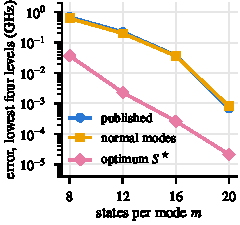
\includegraphics[width=\linewidth]{chapter-2-quantization/figs/kite_levels.pdf}
    \end{minipage}
    \caption{{\bf Product-state coordinates of the $\cos(2\varphi)$ KITE.}
    (a) The $\cos(2\varphi)$ KITE circuit \cite{smithSuperconductingCircuitProtected2020b,Roverch2026experimental}.
    Only the shunted node carries capacitance to ground, so three dynamical modes remain: the compact phase $\varphi$ across $C_S$, plus the extended sum and difference $\varphi_{\Sigma},\varphi_{\Delta}$ of the two upper inductor phases.
    (b) Largest error of the four lowest levels of hierarchical diagonalization with $m$ mean-field eigenstates per mode, one set per well, in three frames.
    We compare the published coordinates $(\varphi,\varphi_\Sigma,\varphi_\Delta)$ of Ref.~\cite{Roverch2026experimental}, the normal modes, and the product-state optimum $S^\star$ of \cref{eq:kite_S_opt}.
    Details of the diagonalization are given in \cref{apx:meanfield}.}
    \label{fig:kite}
\end{figure}

One motivation for normal modes is to make the hierarchical diagonalization of the previous section efficient.
Hierarchical diagonalization solves each mode separately and then diagonalizes the full Hamiltonian in a truncated product of the low-lying single-mode states.
The truncation is accurate when the full system eigenstates are close to the products of single-mode states.
Normal modes remove the quadratic coupling but leave the junction coupling terms, so for a circuit with strong nonlinear coupling, it does not generally achieve this goal.

The $\cos(2\varphi)$ KITE \cite{smithSuperconductingCircuitProtected2020b,Roverch2026experimental} is such a circuit, and we can use an optimization over variable transformations to find an efficient basis for diagonalization.
The cost we consider is the energy of a product of single-mode ground states, evaluated in the full Hamiltonian.
Minimizing it over $S$ is a proxy for how well products of single-mode basis states represent the full ground state.
For a fixed $S$, each mode's ground state is found in a mean-field Hamiltonian, in which the operators of the other modes are replaced by their expectation values.
These expectation values are updated and the single-mode problems re-solved until the product state converges.
An outer optimizer then minimizes the converged energy over $S\in\mathcal A_{\rm relaxed}$, parametrized as in \cref{eq:S_numerical}.
This procedure is inspired by \cite{yagi2012optimized}, which identifies optimized coordinates for anharmonic vibrational structures.
\Cref{apx:meanfield} gives the full construction.

For the KITE at half flux, the optimized frame gives a much better product state than either the published coordinates or the normal modes, and the gain carries over to hierarchical diagonalization.
We take the parameters of Ref.~\cite{Roverch2026experimental}, $E_J=16.83$, $E_{C_J}=4.82$, $E_{C_S}=0.072$ GHz, an inductive energy of $2.54$ GHz per inductor, and junction asymmetry $\epsilon=0.03$, with the flux shared equally over the four inductors.
The ground state is then the doublet of the two $\varphi$ wells, split by 13.5 MHz.
We measure the gap $E_{\rm prod}-E_0$ and the weight of the product state outside the doublet.
Both are evaluated against a reference sparse eigensolve in the published coordinates on 49 charge states for $\varphi$ and 160 grid points for each extended mode, $1{,}254{,}400$ states in all.
The same solve in the optimized coordinates agrees with it to within $10^{-5}$ GHz on the four lowest levels.
In the frame of \cref{fig:kite}(a) both junctions span all three coordinates, and the product state is a poor representation of the ground state, despite the small quadratic coupling, with a gap of 1.44 GHz and 18\% of the weight outside the doublet.
The normal modes remove the quadratic coupling but gain little, with a gap of 1.06 GHz and 17\% of the weight outside the doublet.

The optimized coordinates greatly improve the picture.
Taken relative to $(\varphi,\varphi_\Sigma,\varphi_\Delta)$ with the noncompact columns $C$-normalized,
\begin{align}
S^\star=\begin{pmatrix}1&0.24&0.23\\0&0.70&0.73\\0&-0.57&0.63\end{pmatrix},
\label{eq:kite_S_opt}
\end{align}
reaches a gap of 0.09 GHz with 0.5\% of the weight outside the doublet.
It rotates $(\varphi_\Sigma,\varphi_\Delta)$ by about $40^\circ$ back toward the two arm phases and shears $\varphi$ into both.
Each junction depends on $\varphi$ and essentially one new extended coordinate, with the arguments $\cos(\varphi-1.03\varphi_2'+0.13\varphi_3')$ and $\cos(\varphi+0.11\varphi_2'-1.13\varphi_3')$.
The price is the quadratic coupling that the normal modes had removed.
For hierarchical diagonalization, we keep $m$ eigenstates of each mode's mean-field Hamiltonian, drawn from both wells as described in \cref{apx:meanfield}, and diagonalize the full Hamiltonian in their product.
This basis has $m^3$ states, so at $m=20$ it holds 8000 states, about 160 times fewer than the reference solve.
The largest error of the four lowest levels is about $2\times10^{-5}$ GHz in the optimized coordinates, against about $10^{-3}$ GHz in the other two, and the optimized frame stays one to two orders of magnitude ahead at every $m$ considered.

% =====================================================
\section{Conclusion}\label{sec:conc}
% =====================================================

The topology of a circuit fixes the number and types of modes present but leaves a large family of valid coordinates.
The choice within that family is a modeling decision with consequences.
We have characterized all valid mode-preserving transformations and posed the choice of coordinates as an optimization over them, which can be solved symbolically or numerically for any scalar cost.
The examples show that no single choice serves every task.
The reference coordinates of circuit enumeration, the normal modes, and the product-state coordinates of the KITE all differ, and the last gives up the quadratic decoupling of the normal modes in exchange for a hierarchical basis that is one to two orders of magnitude more accurate.
More generally, the coordinates can and should be tuned to specific applications by supplying the corresponding cost.

Our treatment is restricted to circuits of linear capacitors, inductors, and Josephson junctions, whose potential energy depends on flux alone.
Nonlinear capacitive elements such as quantum phase slip junctions, multiport devices, and non-reciprocal elements such as gyrators require a more general treatment~\cite{osborne_symplectic_2023,OsborneFluxChargeSymmetricTheory2024,salcedoGyratorsSuperconductingCircuit2026,parra-rodriguez2023,smitham2024reciprocallumpedelementsuperconductingcircuits}.
Their energies depend on both flux and charge, and the flux-charge symmetric formalism obtains the Hamiltonian by a symplectic reduction in both sets of variables~\cite{OsborneFluxChargeSymmetricTheory2024,salcedoGyratorsSuperconductingCircuit2026}.
The coordinate freedom is then a family of linear symplectic transformations of fluxes and charges together, rather than the point transformations considered here, for which $\tilde Q=Z^TQ$ follows from the choice of $Z$.
Characterizing the type-preserving subset of that larger family is a natural extension of this work.
